\documentclass[11pt]{article}
\usepackage[notes]{la}
\lamodule{4}{5}{The Dimension of a Vector Space}
\laxdoc{4.3}
\laxdoc{4.4}

\begin{document}

\section{The Dimension of a Vector Space}

\begin{guide}
Pause and think~\ref{4.3-think:manybases} left a question open: can two bases of the same space have different numbers of vectors? Every basis we have met for $\R^2$ had two vectors and every basis for $\R^3$ had three, and in Section 4.4 the coordinate mapping turned a basis with $p$ vectors into a copy of $\R^p$. This section settles the question: the number of vectors in a basis depends only on the space. We call it the \emph{dimension}, and then ask what a single number can do for us. How many vectors can an independent set in a space have? Can we decide whether a set is a basis by \emph{counting} and then checking only one of the two properties? And when we row reduce a matrix, what is the relation between the pivot columns that span $\Col A$ and the free variables that parametrize $\Nul A$?
\end{guide}

\textbf{By the end of this section you should be able to:}
\begin{itemize}
  \item state and use the fact that a set with more vectors than a basis is dependent, and explain why all bases of a space have the same number of vectors;
  \item define the dimension of a finite-dimensional space, give the dimensions of $\R^n$, $\mathbb{P}_n$ and $M_{m\times n}$, and explain why a space such as the space of all polynomials has no finite dimension;
  \item find the dimension of, and a basis for, a subspace of $\R^n$, $\mathbb{P}_n$, $M_{m\times n}$ or a function space that is given by a spanning set, by parameters or by equations;
  \item extend an independent set to a basis and shrink a spanning set to a basis, and use the dimension of a subspace to compare it with the whole space;
  \item use the Basis Theorem to decide whether a set is a basis by counting and checking \emph{one} property, and say where the theorem fails if a hypothesis is dropped;
  \item find $\dim\Nul A$, $\dim\Col A$ and $\dim\Row A$ from an echelon form, and use the Rank Theorem $\rank A+\dim\Nul A=n$ to solve counting problems without any computation;
  \item add the statements about bases, rank and dimension to the Invertible Matrix Theorem and use them to test a square matrix.
\end{itemize}

% ---------------------------------------------------------------------
\subsection*{Counting the vectors in a basis}

The key to everything in this section is a statement about independent sets. In $\R^n$ we know it (Section 1.7): a set of more than $n$ vectors of $\R^n$ is linearly dependent, because the matrix whose columns are the vectors has more columns than rows and therefore a free variable. The coordinate mapping of Section 4.4 lets us carry the statement to every vector space that has a basis.

\begin{thm}{More vectors than a basis}{count}
Let $V$ be a vector space that has a basis $\mathcal{B}=\{\bv{b}_1,\dots,\bv{b}_n\}$ consisting of $n$ vectors. Then every set in $V$ that contains more than $n$ vectors is linearly dependent.
\end{thm}

\begin{proof}
Let $\{\bv{u}_1,\dots,\bv{u}_p\}$ be a set in $V$ with $p>n$. The coordinate vectors $[\bv{u}_1]_{\mathcal{B}},\dots,[\bv{u}_p]_{\mathcal{B}}$ are $p$ vectors in $\R^n$. Since $p>n$, the matrix with these columns has more columns than rows, so it has a column without a pivot and the columns are linearly dependent (Section 1.7). By Theorem~\ref{4.4-thm:transfer}(b), a set in $V$ is independent if and only if its coordinate vectors are independent in $\R^n$. The coordinate vectors are dependent, so $\{\bv{u}_1,\dots,\bv{u}_p\}$ is dependent.
\end{proof}

\begin{think}{What did the proof use?}{morethan}
(a)~Which two facts did the proof combine, one about $\R^n$ and one about the coordinate mapping of $\mathcal{B}$? (b)~The theorem says that more than $n$ vectors are dependent. Does it say that $n$ or fewer vectors are independent? Give an example in $\R^2$. (c)~The vectors $(1,2)$, $(2,4)$ and $(-3,-6)$ lie on a line through $\bv{0}$ in $\R^2$. Without computing, why must any \emph{two} vectors on that line be dependent?
\end{think}

\begin{exmp}{Four polynomials in $\mathbb{P}_2$}{fourP2}
Let $p_1=1+t$, $p_2=2-t+t^2$, $p_3=-3+t^2$ and $p_4=8-t+t^2$. The standard basis $\{1,t,t^2\}$ of $\mathbb{P}_2$ has three vectors, so by Theorem~\ref{thm:count} the four polynomials are dependent, whatever their coefficients are. To find a dependence relation, use the standard coordinates $(1,1,0)$, $(2,-1,1)$, $(-3,0,1)$, $(8,-1,1)$ (Procedure~\ref{4.4-proc:testcoords}):
\begin{align*}
\begin{amat}{cccc}1 & 2 & -3 & 8\\1 & -1 & 0 & -1\\0 & 1 & 1 & 1\end{amat}
&\rops{R_2-R_1}
\begin{amat}{cccc}1 & 2 & -3 & 8\\0 & -3 & 3 & -9\\0 & 1 & 1 & 1\end{amat}
\rops{R_2\leftrightarrow R_3}
\begin{amat}{cccc}1 & 2 & -3 & 8\\0 & 1 & 1 & 1\\0 & -3 & 3 & -9\end{amat}
\\[4pt]
&\rops{R_1-2R_2,\ R_3+3R_2}
\begin{amat}{cccc}1 & 0 & -5 & 6\\0 & 1 & 1 & 1\\0 & 0 & 6 & -6\end{amat}
\rops{\tfrac{1}{6}R_3}
\begin{amat}{cccc}1 & 0 & -5 & 6\\0 & 1 & 1 & 1\\0 & 0 & 1 & -1\end{amat}
\\[4pt]
&\rops{R_1+5R_3,\ R_2-R_3}
\begin{amat}{cccc}1 & 0 & 0 & 1\\0 & 1 & 0 & 2\\0 & 0 & 1 & -1\end{amat}
\end{align*}
Column $4$ has no pivot, so $x_4$ is free and the reduced form reads $\bv{x}=(x_4,\ 2x_4,\ -x_4)$ for the first three weights, which gives the relation among the polynomials
\[
p_4=p_1+2p_2-p_3.
\]
Check: $(1+t)+2(2-t+t^2)-(-3+t^2)=(1+4+3)+(1-2)t+(2-1)t^2=8-t+t^2$. \ $\checkmark$ The first three polynomials are independent (pivots in columns $1$, $2$, $3$), so $\{p_1,p_2,p_3\}$ is a basis of $\mathbb{P}_2$: the dependence of the full set is caused by the fourth polynomial alone.
\end{exmp}

\begin{exmp}{Three functions in a two-vector space}{funcs}
The functions $\cos t$ and $\sin t$ form a basis for $H=\Span\{\cos t,\sin t\}$ (Example~\ref{4.3-ex:sincos}). Take $f_1=2\cos t-\sin t$, $f_2=\cos t+3\sin t$, $f_3=5\cos t+\sin t$, all in $H$. By Theorem~\ref{thm:count} the three functions are dependent. Their coordinates in the basis $\{\cos t,\sin t\}$ are $(2,-1)$, $(1,3)$, $(5,1)$:
\begin{align*}
\begin{amat}{ccc}2 & 1 & 5\\-1 & 3 & 1\end{amat}
&\rops{R_1\leftrightarrow R_2}
\begin{amat}{ccc}-1 & 3 & 1\\2 & 1 & 5\end{amat}
\rops{-R_1}
\begin{amat}{ccc}1 & -3 & -1\\2 & 1 & 5\end{amat}
\\[4pt]
&\rops{R_2-2R_1}
\begin{amat}{ccc}1 & -3 & -1\\0 & 7 & 7\end{amat}
\rops{\tfrac{1}{7}R_2}
\begin{amat}{ccc}1 & -3 & -1\\0 & 1 & 1\end{amat}
\\[4pt]
&\rops{R_1+3R_2}
\begin{amat}{ccc}1 & 0 & 2\\0 & 1 & 1\end{amat}
\end{align*}
Here $x_3$ is free and the reduced form gives $x_1=-2x_3$, $x_2=-x_3$. With $x_3=1$: $-2f_1-f_2+f_3=\bv{0}$, that is $f_3=2f_1+f_2$. Check: $2(2\cos t-\sin t)+(\cos t+3\sin t)=5\cos t+\sin t$. \ $\checkmark$
\end{exmp}

\begin{exmp}{Three vectors in a plane inside $\R^3$}{planeH}
Let $H=\{\bv{x}\in\R^3:\ x_1-2x_2+x_3=0\}$ with the basis $\bv{b}_1=(2,1,0)$, $\bv{b}_2=(-1,0,1)$ of Example~\ref{4.4-ex:plane}. The vectors $\bv{u}_1=(3,2,1)$, $\bv{u}_2=(1,1,1)$, $\bv{u}_3=(4,1,-2)$ are in $H$ (the equation holds: $3-4+1=0$, $1-2+1=0$, $4-2-2=0$). Three vectors \emph{can} be independent in $\R^3$, but $H$ has a basis of two vectors, so by Theorem~\ref{thm:count} these three are dependent. The coordinates relative to $\{\bv{b}_1,\bv{b}_2\}$ are the second and third entries (Pause and think~\ref{4.4-think:freevars}): $(2,1)$, $(1,1)$, $(1,-2)$.
\begin{align*}
\begin{amat}{ccc}2 & 1 & 1\\1 & 1 & -2\end{amat}
&\rops{R_1\leftrightarrow R_2}
\begin{amat}{ccc}1 & 1 & -2\\2 & 1 & 1\end{amat}
\rops{R_2-2R_1}
\begin{amat}{ccc}1 & 1 & -2\\0 & -1 & 5\end{amat}
\\[4pt]
&\rops{-R_2}
\begin{amat}{ccc}1 & 1 & -2\\0 & 1 & -5\end{amat}
\rops{R_1-R_2}
\begin{amat}{ccc}1 & 0 & 3\\0 & 1 & -5\end{amat}
\end{align*}
With $x_3=1$ we get $x_1=-3$ and $x_2=5$, so
\[
-3\bv{u}_1+5\bv{u}_2+\bv{u}_3=-3\begin{bmatrix}3\\2\\1\end{bmatrix}+5\begin{bmatrix}1\\1\\1\end{bmatrix}+\begin{bmatrix}4\\1\\-2\end{bmatrix}=\begin{bmatrix}0\\0\\0\end{bmatrix}.
\]
The ambient space $\R^3$ has room for three independent vectors, but the plane does not: what counts is the space in which the vectors live, here $H$.
\end{exmp}

% Figure 1 sits after the corollary below

\begin{thm}{All bases have the same number of vectors}{samesize}
Let $V$ be a vector space with a basis of $n$ vectors.
\begin{enumerate}[label=(\alph*),itemsep=1pt]
  \item Every basis of $V$ has exactly $n$ vectors.
  \item Every linearly independent set in $V$ has at most $n$ vectors, and every spanning set for $V$ has at least $n$ vectors.
\end{enumerate}
\end{thm}

\begin{proof}
Let $\mathcal{B}$ be the given basis (with $n$ vectors) and let $\mathcal{C}$ be another basis, with $p$ vectors. (a)~Since $\mathcal{C}$ is independent, Theorem~\ref{thm:count} applied to $\mathcal{B}$ shows that $\mathcal{C}$ cannot have more than $n$ vectors: $p\le n$. Since $\mathcal{B}$ is independent, the same theorem applied to the basis $\mathcal{C}$ shows $n\le p$. Hence $p=n$. (b)~The first statement is Theorem~\ref{thm:count}. If a set $S$ spans $V$, it contains a basis of $V$ (Theorem~\ref{4.3-thm:sst}), which has $n$ vectors by (a); so $S$ has at least $n$ vectors.
\end{proof}

This is the answer to Pause and think~\ref{4.3-think:manybases}: \emph{no}, two bases of the same space never have different numbers of vectors. The proof is short because all the work was done in Section 4.4: a basis lets us treat the space as $\R^n$ (Theorem~\ref{4.4-thm:coordmap}), and the count in $\R^n$ is the count of Section 1.7.

\begin{think}{Pause and think~\ref{4.3-think:manybases} revisited}{manybases}
(a)~Use Theorem~\ref{thm:samesize} to explain why no basis of $\R^3$ can have $2$ vectors and none can have $4$. (b)~The free-variable basis of $\Nul A$ (Theorem~\ref{4.3-thm:nulbasis}) depends on how we label the free variables; a student finds a different basis of the same null space by taking, say, a pair of different vectors in the plane. Must the two bases have the same number of vectors, and why? (c)~Is the statement ``a vector space has a basis with $n$ vectors for exactly one $n$'' still true for the zero space? What should its basis be?
\end{think}

\begin{center}
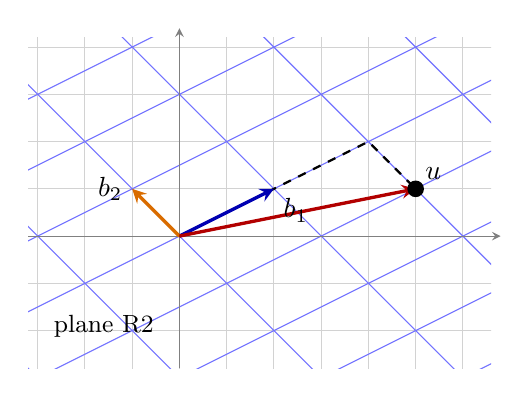
\begin{tikzpicture}[x=0.6cm,y=0.6cm,>=stealth]
  \begin{scope}
    \clip (-3.2,-2.8) rectangle (6.6,4.2);
    \draw[gray!35] (-6,-4) grid[step=1] (8,6);
    \begin{scope}[cm={2,1,-1,1,(0,0)}]
      \draw[blue!55] (-6,-6) grid[step=1] (6,6);
    \end{scope}
  \end{scope}
  \draw[->,gray] (-3.2,0)--(6.8,0);
  \draw[->,gray] (0,-2.8)--(0,4.4);
  \draw[dashed,thick] (0,0)--(4,2)--(5,1);
  \draw[->,very thick,blue!70!black] (0,0)--(2,1);
  \draw[->,very thick,orange!85!black] (0,0)--(-1,1);
  \draw[->,very thick,red!70!black] (0,0)--(5,1);
  \fill (5,1) circle (3pt);
  \node[below right] at (2,1) {$b_1$};
  \node[left] at (-1,1) {$b_2$};
  \node[above right] at (5,1) {$u$};
  \node at (-1.6,-1.9) {\small plane R2};
\end{tikzpicture}
\end{center}

\textbf{Figure 1.} Three vectors in a plane. The plane has the basis $\bv{b}_1=(2,1)$, $\bv{b}_2=(-1,1)$ (blue grid), so by Theorem~\ref{thm:count} any third vector is dependent on them. Here $\bv{u}=(5,1)$ is reached by two steps along $\bv{b}_1$ (dashed) and one step \emph{backwards} along $\bv{b}_2$: $\bv{u}=2\bv{b}_1-\bv{b}_2$, that is $2\bv{b}_1-\bv{b}_2-\bv{u}=\bv{0}$. The two grid directions are enough to reach every point, so a third direction is always redundant.

% ---------------------------------------------------------------------
\subsection*{Dimension}

\begin{defn}{Dimension}{dim}
If a vector space $V$ is spanned by a finite set, $V$ is \emph{finite-dimensional}, and the \emph{dimension} of $V$, written $\dim V$, is the number of vectors in a basis for $V$. The dimension of the zero space $\{\bv{0}\}$ is defined to be $0$ (its basis is the empty set). If $V$ is not spanned by any finite set, $V$ is \emph{infinite-dimensional}.
\end{defn}

The definition makes sense because of Theorem~\ref{thm:samesize}: a finite spanning set contains a basis (Theorem~\ref{4.3-thm:sst}), and every basis has the same number of vectors, so ``the number of vectors in a basis'' is a single number attached to $V$. Dimension counts the independent directions in the space, as in Figure~1: a plane has two, a line has one.

\begin{exmp}{The dimensions of the standard spaces}{stddims}
\textbf{(a)} $\dim\R^n=n$: the standard basis $\{\bv{e}_1,\dots,\bv{e}_n\}$ has $n$ vectors (Example~\ref{4.3-ex:standard}). \textbf{(b)} $\dim\mathbb{P}_n=n+1$: a basis is $\{1,t,t^2,\dots,t^n\}$. So $\dim\mathbb{P}_2=3$ and $\dim\mathbb{P}_5=6$. \textbf{(c)} $\dim M_{m\times n}=mn$: a basis consists of the $mn$ matrices with a single entry $1$ and all other entries $0$. So $\dim M_{2\times2}=4$ and $\dim M_{2\times3}=6$. \textbf{(d)} $\dim\{\bv{0}\}=0$. The spaces $\R^3$ and $\mathbb{P}_2$ are different spaces, but both have dimension $3$; so do $M_{2\times2}$ and $\R^4$ (dimension $4$). The coordinate mapping of Section 4.4 is the way to move between spaces of the same dimension, and $\Span\{\cos t,\sin t\}$ has dimension $2$ like $\R^2$.
\end{exmp}

\begin{exmp}{A space with no finite dimension}{infdim}
Let $\mathbb{P}$ be the space of \emph{all} polynomials. Suppose $\mathbb{P}$ had a basis of $n$ vectors for some number $n$. The $n+1$ polynomials $1,t,t^2,\dots,t^n$ are linearly independent (a polynomial is the zero polynomial only if every coefficient is $0$), and they are $n+1>n$ vectors of $\mathbb{P}$. This contradicts Theorem~\ref{thm:count}. So there is no basis with finitely many vectors, and no finite set spans $\mathbb{P}$ (a finite spanning set would contain a finite basis): $\mathbb{P}$ is infinite-dimensional. The same argument applies to any vector space that contains all the polynomials, for example the space of all functions $\R\to\R$ or the space of continuous functions: each is infinite-dimensional. Infinite-dimensional spaces are important in analysis, but they are not the subject of this course: from now on ``dimension'' means finite dimension.
\end{exmp}

\begin{kc}{Dimension of the standard spaces}{dimstd}
(a)~Find $\dim\R^6$, $\dim\mathbb{P}_5$, $\dim M_{3\times4}$ and $\dim M_{2\times2}$. (b)~Can $5$ vectors form a basis of $\R^4$? Can $3$? (c)~The set of polynomials in $\mathbb{P}_3$ with $p(0)=0$ is a subspace with basis $\{t,t^2,t^3\}$. What is its dimension? (d)~Does $\mathbb{P}_2$ have a basis of $4$ polynomials?
\end{kc}

% ---------------------------------------------------------------------
\subsection*{The dimension of a subspace}

A subspace is usually described in one of three ways: by a spanning set, by parameters (which is a spanning set in disguise), or by equations. In each case the dimension is found by counting the pivots of a matrix.

\begin{proc}{The dimension of a subspace $H$}{dimH}
\begin{enumerate}
  \item \emph{Get a spanning set.} If $H$ is given by a spanning set, use it. If $H$ is given by parameters, the vectors multiplying the parameters span $H$. If $H$ is given by equations, solve the homogeneous system and write the solution in parametric vector form (Procedure~\ref{4.3-proc:cond}); the vectors multiplying the free variables span $H$.
  \item \emph{Write the vectors as coordinate columns} relative to a standard basis of the ambient space (the entries of vectors in $\R^n$, the coefficients of polynomials, the entries of matrices read row by row), make them the columns of a matrix and row reduce.
  \item \emph{Count.} The pivot columns give a basis of $H$ (Theorem~\ref{4.3-thm:colbasis} and Theorem~\ref{4.4-thm:transfer}), so $\dim H$ is the number of pivots. For a system of equations, $\dim H$ is the number of free variables, that is (number of unknowns) $-$ (number of pivots of the coefficient matrix).
\end{enumerate}
\end{proc}

\begin{exmp}{The span of three vectors in $\R^4$}{spanR4}
Let $\bv{v}_1=(1,2,-1,3)$, $\bv{v}_2=(-2,5,-4,-1)$, $\bv{v}_3=(5,-8,7,5)$ and $H=\Span\{\bv{v}_1,\bv{v}_2,\bv{v}_3\}$. Find $\dim H$ and a basis.
\begin{align*}
\begin{amat}{ccc}1 & -2 & 5\\2 & 5 & -8\\-1 & -4 & 7\\3 & -1 & 5\end{amat}
&\rops{R_2-2R_1,\ R_3+R_1,\ R_4-3R_1}
\begin{amat}{ccc}1 & -2 & 5\\0 & 9 & -18\\0 & -6 & 12\\0 & 5 & -10\end{amat}
\rops{R_2\leftrightarrow R_4}
\begin{amat}{ccc}1 & -2 & 5\\0 & 5 & -10\\0 & -6 & 12\\0 & 9 & -18\end{amat}
\\[4pt]
&\rops{\tfrac{1}{5}R_2}
\begin{amat}{ccc}1 & -2 & 5\\0 & 1 & -2\\0 & -6 & 12\\0 & 9 & -18\end{amat}
\rops{R_1+2R_2,\ R_3+6R_2,\ R_4-9R_2}
\begin{amat}{ccc}1 & 0 & 1\\0 & 1 & -2\\0 & 0 & 0\\0 & 0 & 0\end{amat}
\end{align*}
There are two pivots, in columns $1$ and $2$. So $\{\bv{v}_1,\bv{v}_2\}$ is a basis for $H$ and $\dim H=2$. Column $3$ of the reduced form is $(1,-2)$, so $\bv{v}_3=\bv{v}_1-2\bv{v}_2$. Check: $(1,2,-1,3)-2(-2,5,-4,-1)=(5,-8,7,5)$. \ $\checkmark$ A spanning set of three vectors gave a space of dimension $2$: dimension is the number of \emph{independent} vectors, not the number of vectors that were listed.
\end{exmp}

\begin{exmp}{Three parameters, dimension two}{param}
Let $H=\{(a+b,\ b-c,\ a+c,\ 2a+b+c):\ a,b,c \text{ in } \R\}$. Separating the parameters,
\[
\begin{bmatrix}a+b\\b-c\\a+c\\2a+b+c\end{bmatrix}=a\begin{bmatrix}1\\0\\1\\2\end{bmatrix}+b\begin{bmatrix}1\\1\\0\\1\end{bmatrix}+c\begin{bmatrix}0\\-1\\1\\1\end{bmatrix},
\]
so $H=\Span\{\bv{u}_1,\bv{u}_2,\bv{u}_3\}$ with $\bv{u}_1=(1,0,1,2)$, $\bv{u}_2=(1,1,0,1)$, $\bv{u}_3=(0,-1,1,1)$.
\begin{align*}
\begin{amat}{ccc}1 & 1 & 0\\0 & 1 & -1\\1 & 0 & 1\\2 & 1 & 1\end{amat}
&\rops{R_3-R_1,\ R_4-2R_1}
\begin{amat}{ccc}1 & 1 & 0\\0 & 1 & -1\\0 & -1 & 1\\0 & -1 & 1\end{amat}
\rops{R_1-R_2,\ R_3+R_2,\ R_4+R_2}
\begin{amat}{ccc}1 & 0 & 1\\0 & 1 & -1\\0 & 0 & 0\\0 & 0 & 0\end{amat}
\end{align*}
The pivots are in columns $1$ and $2$ and column $3$ is $(1,-1)$, so $\bv{u}_3=\bv{u}_1-\bv{u}_2$ (check: $(1,0,1,2)-(1,1,0,1)=(0,-1,1,1)$). \ $\checkmark$ The set $\{\bv{u}_1,\bv{u}_2\}$ is a basis for $H$ and $\dim H=2$, although $H$ was described with three parameters. A parametrization with $k$ parameters gives a subspace of dimension \emph{at most} $k$, with equality exactly when the vectors multiplying the parameters are independent.
\end{exmp}

\begin{exmp}{A subspace of $\R^4$ given by equations}{eqns}
Let $H$ be the set of solutions of
\[
x_1+x_2+x_3+x_4=0,\qquad x_1-x_3=0,\qquad 2x_1+x_2+x_4=0.
\]
\begin{align*}
\begin{amat}{cccc}1 & 1 & 1 & 1\\1 & 0 & -1 & 0\\2 & 1 & 0 & 1\end{amat}
&\rops{R_2-R_1,\ R_3-2R_1}
\begin{amat}{cccc}1 & 1 & 1 & 1\\0 & -1 & -2 & -1\\0 & -1 & -2 & -1\end{amat}
\rops{-R_2}
\begin{amat}{cccc}1 & 1 & 1 & 1\\0 & 1 & 2 & 1\\0 & -1 & -2 & -1\end{amat}
\\[4pt]
&\rops{R_1-R_2,\ R_3+R_2}
\begin{amat}{cccc}1 & 0 & -1 & 0\\0 & 1 & 2 & 1\\0 & 0 & 0 & 0\end{amat}
\end{align*}
The coefficient matrix has pivots in columns $1$ and $2$ only; $x_3$ and $x_4$ are free. So $x_1=x_3$ and $x_2=-2x_3-x_4$, and
\[
\bv{x}=x_3\begin{bmatrix}1\\-2\\1\\0\end{bmatrix}+x_4\begin{bmatrix}0\\-1\\0\\1\end{bmatrix}.
\]
The two vectors are independent (look at the free-variable entries), so $\dim H=4-2=2$. Notice that the third equation is the sum of the first two; it adds nothing, and the number of \emph{pivots}, $2$, is what counts, not the number of equations, $3$. Check that $(1,-2,1,0)$ satisfies all three equations: $1-2+1+0=0$, $1-1=0$, $2-2+0=0$. \ $\checkmark$
\end{exmp}

\begin{exmp}{A subspace of $\mathbb{P}_3$ spanned by five polynomials}{spanP3}
Let $c_1=1+2t$, $c_2=t+t^2$, $c_3=1-t-3t^2$, $c_4=t^2+t^3$, $c_5=1+3t+2t^2+t^3$ and $H=\Span\{c_1,\dots,c_5\}$. The standard coordinates (coefficients of $1,t,t^2,t^3$) are $(1,2,0,0)$, $(0,1,1,0)$, $(1,-1,-3,0)$, $(0,0,1,1)$, $(1,3,2,1)$.
\begin{align*}
\begin{amat}{ccccc}1 & 0 & 1 & 0 & 1\\2 & 1 & -1 & 0 & 3\\0 & 1 & -3 & 1 & 2\\0 & 0 & 0 & 1 & 1\end{amat}
&\rops{R_2-2R_1}
\begin{amat}{ccccc}1 & 0 & 1 & 0 & 1\\0 & 1 & -3 & 0 & 1\\0 & 1 & -3 & 1 & 2\\0 & 0 & 0 & 1 & 1\end{amat}
\\[4pt]
&\rops{R_3-R_2}
\begin{amat}{ccccc}1 & 0 & 1 & 0 & 1\\0 & 1 & -3 & 0 & 1\\0 & 0 & 0 & 1 & 1\\0 & 0 & 0 & 1 & 1\end{amat}
\\[4pt]
&\rops{R_4-R_3}
\begin{amat}{ccccc}1 & 0 & 1 & 0 & 1\\0 & 1 & -3 & 0 & 1\\0 & 0 & 0 & 1 & 1\\0 & 0 & 0 & 0 & 0\end{amat}
\end{align*}
The pivots are in columns $1$, $2$, $4$, so $\{c_1,c_2,c_4\}$ is a basis for $H$ and $\dim H=3$. The other columns give the relations $c_3=c_1-3c_2$ and $c_5=c_1+c_2+c_4$. Check: $(1+2t)-3(t+t^2)=1-t-3t^2$, and $(1+2t)+(t+t^2)+(t^2+t^3)=1+3t+2t^2+t^3$. \ $\checkmark$ Since $\dim\mathbb{P}_3=4$, the subspace $H$ is not all of $\mathbb{P}_3$ (Theorem~\ref{thm:subspace} below makes this precise).
\end{exmp}

\begin{exmp}{Three subspaces of $M_{2\times2}$}{M2cond}
Write a matrix as $\begin{bmatrix}a&b\\c&d\end{bmatrix}$; its standard coordinates are $(a,b,c,d)$ and $\dim M_{2\times2}=4$.

\textbf{(a) Symmetric matrices} ($b=c$). One equation on four unknowns, so $\dim=4-1=3$; a basis is $\begin{bmatrix}1&0\\0&0\end{bmatrix}$, $\begin{bmatrix}0&1\\1&0\end{bmatrix}$, $\begin{bmatrix}0&0\\0&1\end{bmatrix}$.

\textbf{(b) Matrices with trace $0$} ($a+d=0$). One equation, $\dim=3$; $a=-d$ with $b,c,d$ free gives the basis $\begin{bmatrix}1&0\\0&-1\end{bmatrix}$, $\begin{bmatrix}0&1\\0&0\end{bmatrix}$, $\begin{bmatrix}0&0\\1&0\end{bmatrix}$.

\textbf{(c) Matrices whose row sums and column sums are all zero.} The four equations $a+b=0$, $c+d=0$, $a+c=0$, $b+d=0$ have the coefficient matrix below:
\begin{align*}
\begin{amat}{cccc}1 & 1 & 0 & 0\\0 & 0 & 1 & 1\\1 & 0 & 1 & 0\\0 & 1 & 0 & 1\end{amat}
&\rops{R_3-R_1}
\begin{amat}{cccc}1 & 1 & 0 & 0\\0 & 0 & 1 & 1\\0 & -1 & 1 & 0\\0 & 1 & 0 & 1\end{amat}
\rops{R_2\leftrightarrow R_3}
\begin{amat}{cccc}1 & 1 & 0 & 0\\0 & -1 & 1 & 0\\0 & 0 & 1 & 1\\0 & 1 & 0 & 1\end{amat}
\\[4pt]
&\rops{-R_2}
\begin{amat}{cccc}1 & 1 & 0 & 0\\0 & 1 & -1 & 0\\0 & 0 & 1 & 1\\0 & 1 & 0 & 1\end{amat}
\rops{R_1-R_2,\ R_4-R_2}
\begin{amat}{cccc}1 & 0 & 1 & 0\\0 & 1 & -1 & 0\\0 & 0 & 1 & 1\\0 & 0 & 1 & 1\end{amat}
\\[4pt]
&\rops{R_1-R_3,\ R_2+R_3,\ R_4-R_3}
\begin{amat}{cccc}1 & 0 & 0 & -1\\0 & 1 & 0 & 1\\0 & 0 & 1 & 1\\0 & 0 & 0 & 0\end{amat}
\end{align*}
Only three pivots: the fourth equation is redundant (the sum of the first two equals the sum of the last two). So $\dim=4-3=1$. The free variable is $d$, and $a=d$, $b=-d$, $c=-d$: the subspace is spanned by $\begin{bmatrix}1&-1\\-1&1\end{bmatrix}$, and $\dim=1$.
\end{exmp}

\begin{exmp}{Polynomials with two prescribed roots}{polycond}
Let $H=\{p\in\mathbb{P}_3:\ p(1)=0\ \text{and}\ p(-1)=0\}$. Write $p(t)=a+bt+ct^2+dt^3$. The two conditions are $a+b+c+d=0$ and $a-b+c-d=0$.
\begin{align*}
\begin{amat}{cccc}1 & 1 & 1 & 1\\1 & -1 & 1 & -1\end{amat}
&\rops{R_2-R_1}
\begin{amat}{cccc}1 & 1 & 1 & 1\\0 & -2 & 0 & -2\end{amat}
\rops{-\tfrac{1}{2}R_2}
\begin{amat}{cccc}1 & 1 & 1 & 1\\0 & 1 & 0 & 1\end{amat}
\\[4pt]
&\rops{R_1-R_2}
\begin{amat}{cccc}1 & 0 & 1 & 0\\0 & 1 & 0 & 1\end{amat}
\end{align*}
Pivots in columns $1$ and $2$; $c$ and $d$ are free, with $a=-c$ and $b=-d$. So $p(t)=c(t^2-1)+d(t^3-t)$, a basis for $H$ is $\{t^2-1,\ t^3-t\}$ and $\dim H=4-2=2$. Check: both polynomials vanish at $t=1$ and $t=-1$. \ $\checkmark$ Each independent condition lowered the dimension of $\mathbb{P}_3$ by one.
\end{exmp}

\begin{exmp}{Functions satisfying a hidden identity}{trig}
Let $H=\Span\{1,\ \cos^2t,\ \cos2t\}$. The double-angle identity $\cos2t=2\cos^2t-1$ says that the third function is a combination of the first two, so by the Spanning Set Theorem (Theorem~\ref{4.3-thm:sst}) the third can be deleted: $H=\Span\{1,\cos^2t\}$. The remaining two functions are independent: if $c_1\cdot1+c_2\cos^2t=0$ for all $t$, then $t=\pi/2$ gives $c_1=0$ and $t=0$ gives $c_1+c_2=0$, so $c_2=0$. Hence $\{1,\cos^2t\}$ is a basis for $H$, and $\dim H=2$. Three functions, dimension $2$.
\end{exmp}

\begin{kc}{Dimension of a subspace}{subdim}
Find the dimension of each subspace and give a basis. (a)~$\Span\{(1,1,0),(0,1,1),(1,2,1)\}$ in $\R^3$. (b)~$\{(a,\ b,\ a+b,\ a-b):\ a,b \text{ in } \R\}$ in $\R^4$. (c)~The solutions in $\R^3$ of $x_1+x_2+x_3=0$ and $x_1-x_2=0$. (d)~The matrices $\begin{bmatrix}a&b\\c&d\end{bmatrix}$ in $M_{2\times2}$ with $a=d$.
\end{kc}

\begin{think}{Parameters, equations and dimension}{params}
(a)~In Example~\ref{ex:param} there were three parameters but $\dim H=2$. What property of the three vectors would make ``number of parameters $=$ dimension'' true? (b)~A homogeneous system in $5$ unknowns has $3$ pivots in its coefficient matrix. What is the dimension of its solution set? Does it depend on the number of equations? (c)~A subspace of $\R^6$ is described by $4$ equations. Is its dimension necessarily $6-4=2$? What is true instead?
\end{think}

% ---------------------------------------------------------------------
\subsection*{Subspaces of a finite-dimensional space}

\begin{thm}{Dimension of a subspace}{subspace}
Let $H$ be a subspace of a finite-dimensional vector space $V$.
\begin{enumerate}[label=(\alph*),itemsep=1pt]
  \item Every linearly independent set in $H$ can be extended, if necessary, to a basis for $H$.
  \item $H$ is finite-dimensional and $\dim H\le\dim V$.
  \item If $\dim H=\dim V$, then $H=V$.
\end{enumerate}
\end{thm}

\begin{proof}
Let $n=\dim V$. (a)~Let $S=\{\bv{v}_1,\dots,\bv{v}_k\}$ be independent in $H$ (possibly $k=0$). If $S$ spans $H$, it is a basis. If not, choose $\bv{w}$ in $H$ that is not in $\Span S$. Then $S\cup\{\bv{w}\}$ is independent: in a relation $c_1\bv{v}_1+\cdots+c_k\bv{v}_k+c\bv{w}=\bv{0}$ we must have $c=0$ (otherwise $\bv{w}$ would be a combination of the $\bv{v}_i$), and then $c_1=\cdots=c_k=0$ by the independence of $S$. Repeat with the larger set. Every independent set in $V$ has at most $n$ vectors (Theorem~\ref{thm:samesize}(b)), so the process stops after at most $n-k$ steps, and it stops only when the set spans $H$. (b)~Take $k=0$ in (a): $H$ has a basis, with at most $n$ vectors. (c)~Let $\dim H=n$. A basis of $H$ is an independent set of $n$ vectors in $V$; apply (a) to $V$ itself: this set extends to a basis of $V$, which has exactly $n$ vectors, so nothing has to be added, and the $n$ vectors already span $V$. Hence $H=V$.
\end{proof}

The theorem formalizes what Figure~1 suggests: a subspace cannot have more independent directions than the space around it, and if it has as many, it is the whole space. In $\R^3$ the possible subspaces are therefore as follows.

\begin{exmp}{All subspaces of $\R^2$ and $\R^3$}{R3subs}
A subspace $H$ of $\R^3$ has $\dim H\in\{0,1,2,3\}$ by Theorem~\ref{thm:subspace}(b), and $H$ is spanned by a basis of that many independent vectors: $\dim H=0$ gives $\{\bv{0}\}$; $\dim H=1$ gives a line through the origin, $\Span\{\bv{v}\}$ with $\bv{v}\ne\bv{0}$; $\dim H=2$ gives a plane through the origin, $\Span\{\bv{v},\bv{w}\}$ with $\bv{v},\bv{w}$ independent; $\dim H=3$ gives all of $\R^3$ by Theorem~\ref{thm:subspace}(c). In $\R^2$ the subspaces are $\{\bv{0}\}$, lines through the origin, and $\R^2$. For example the set $\{(x_1,x_2):\ x_2=x_1^2\}$ is not a subspace of $\R^2$, and a quick way to see it is to notice that it contains $(1,1)$ and $(2,4)$, which are independent, so a subspace containing both would be all of $\R^2$ and would contain $(1,0)$, which is not on the curve. A subspace of $\R^3$ that contains $(1,2,0)$ and $(0,1,1)$ is at least a plane; if it also contains $(1,3,1)=(1,2,0)+(0,1,1)$ it is exactly that plane, but if it contains $(1,0,0)$ as well it is all of $\R^3$, because the three vectors are independent.
\end{exmp}

\begin{think}{Same dimension, same subspace?}{equal}
(a)~Part (c) of Theorem~\ref{thm:subspace} says that a subspace of the same dimension as $V$ is $V$. Use parts (b) and (c) to explain why a plane through the origin of $\R^3$ is not $\R^3$, and why it cannot contain three independent vectors. (b)~In the space $\mathbb{P}$ of all polynomials let $H=\{p:\ p(0)=0\}$, the polynomials with no constant term. It is a subspace, and it is not all of $\mathbb{P}$ (the constant polynomial $1$ is not in $H$). Its basis is $t,t^2,t^3,\dots$ without end. Why does part (c) not apply? (c)~Which step of the proof of (c) used that $V$ has a finite dimension?
\end{think}

% ---------------------------------------------------------------------
\subsection*{Extending and shrinking to a basis}

Part (a) of Theorem~\ref{thm:subspace} says that an independent set can always be made into a basis by adding vectors. The Spanning Set Theorem (Theorem~\ref{4.3-thm:sst}) says that a spanning set can always be made into a basis by removing vectors. Both can be done by one row reduction.

\begin{proc}{Extending an independent set to a basis}{extend}
Let $S=\{\bv{v}_1,\dots,\bv{v}_k\}$ be independent in a space $V$ and let $E=\{\bv{e}_1,\dots,\bv{e}_m\}$ be a set that spans $V$ (for example a known basis of $V$, or of a subspace).
\begin{enumerate}
  \item Write all vectors as coordinate columns relative to a standard basis and form the matrix $\begin{bmatrix}\bv{v}_1&\cdots&\bv{v}_k&\bv{e}_1&\cdots&\bv{e}_m\end{bmatrix}$.
  \item Row reduce. The pivot columns form a basis for the column space, which corresponds to $\Span(S\cup E)=V$ (Theorem~\ref{4.3-thm:colbasis} and Theorem~\ref{4.4-thm:transfer}).
  \item The first $k$ columns are pivot columns (they are independent, so none is a combination of the columns before it). The pivot columns among the last $m$ are the vectors to add.
\end{enumerate}
\end{proc}

\begin{exmp}{Extending two vectors to a basis of $\R^4$}{extendR4}
The vectors $\bv{v}_1=(1,2,0,1)$ and $\bv{v}_2=(0,1,1,0)$ are independent ($\bv{v}_2$ is not a multiple of $\bv{v}_1$). Extend them to a basis for $\R^4$ using the standard basis.
\begin{align*}
\begin{amat}{cc|cccc}1 & 0 & 1 & 0 & 0 & 0\\2 & 1 & 0 & 1 & 0 & 0\\0 & 1 & 0 & 0 & 1 & 0\\1 & 0 & 0 & 0 & 0 & 1\end{amat}
&\rops{R_2-2R_1,\ R_4-R_1}
\begin{amat}{cc|cccc}1 & 0 & 1 & 0 & 0 & 0\\0 & 1 & -2 & 1 & 0 & 0\\0 & 1 & 0 & 0 & 1 & 0\\0 & 0 & -1 & 0 & 0 & 1\end{amat}
\\[4pt]
&\rops{R_3-R_2}
\begin{amat}{cc|cccc}1 & 0 & 1 & 0 & 0 & 0\\0 & 1 & -2 & 1 & 0 & 0\\0 & 0 & 2 & -1 & 1 & 0\\0 & 0 & -1 & 0 & 0 & 1\end{amat}
\end{align*}
The pivot columns are $1,2,3,4$, so $\{\bv{v}_1,\bv{v}_2,\bv{e}_1,\bv{e}_2\}$ is a basis for $\R^4$. The columns of $\bv{e}_3$ and $\bv{e}_4$ are combinations of the earlier pivot columns, the entries of the last two reduced columns give the weights, and they are not needed. For instance column $5$ is $(0,1,0,-1)$ in the pivot columns, so $\bv{e}_3=\bv{v}_2-\bv{e}_2$: check $(0,1,1,0)-(0,1,0,0)=(0,0,1,0)$. \ $\checkmark$ Two vectors had to be added, since $\dim\R^4-2=2$.
\end{exmp}

\begin{exmp}{Extending two polynomials to a basis of $\mathbb{P}_3$}{extendP3}
Let $q_1=1+t+t^2+t^3$ and $q_2=t+2t^2$. Standard coordinates: $(1,1,1,1)$ and $(0,1,2,0)$, and the standard basis $1,t,t^2,t^3$ of $\mathbb{P}_3$ is added.
\begin{align*}
\begin{amat}{cc|cccc}1 & 0 & 1 & 0 & 0 & 0\\1 & 1 & 0 & 1 & 0 & 0\\1 & 2 & 0 & 0 & 1 & 0\\1 & 0 & 0 & 0 & 0 & 1\end{amat}
&\rops{R_2-R_1,\ R_3-R_1,\ R_4-R_1}
\begin{amat}{cc|cccc}1 & 0 & 1 & 0 & 0 & 0\\0 & 1 & -1 & 1 & 0 & 0\\0 & 2 & -1 & 0 & 1 & 0\\0 & 0 & -1 & 0 & 0 & 1\end{amat}
\\[4pt]
&\rops{R_3-2R_2}
\begin{amat}{cc|cccc}1 & 0 & 1 & 0 & 0 & 0\\0 & 1 & -1 & 1 & 0 & 0\\0 & 0 & 1 & -2 & 1 & 0\\0 & 0 & -1 & 0 & 0 & 1\end{amat}
\end{align*}
The pivot columns are $1,2,3,4$. So $\{q_1,\ q_2,\ 1,\ t\}$ is a basis for $\mathbb{P}_3$. (A different choice of the spanning set $E$ would produce a different basis; all of them have $4$ vectors.)
\end{exmp}

\begin{exmp}{Extending to a basis of a subspace}{extendH}
Let $H=\{\bv{x}\in\R^4:\ x_1+x_2+x_3+x_4=0\}$. Its free-variable basis is $\bv{g}_1=(-1,1,0,0)$, $\bv{g}_2=(-1,0,1,0)$, $\bv{g}_3=(-1,0,0,1)$, so $\dim H=3$. The vectors $\bv{s}_1=(1,-1,0,0)$ and $\bv{s}_2=(0,1,-1,0)$ are in $H$ and independent. Extend $\{\bv{s}_1,\bv{s}_2\}$ to a basis for $H$ using $\{\bv{g}_1,\bv{g}_2,\bv{g}_3\}$:
\begin{align*}
\begin{amat}{cc|ccc}1 & 0 & -1 & -1 & -1\\-1 & 1 & 1 & 0 & 0\\0 & -1 & 0 & 1 & 0\\0 & 0 & 0 & 0 & 1\end{amat}
&\rops{R_2+R_1}
\begin{amat}{cc|ccc}1 & 0 & -1 & -1 & -1\\0 & 1 & 0 & -1 & -1\\0 & -1 & 0 & 1 & 0\\0 & 0 & 0 & 0 & 1\end{amat}
\\[4pt]
&\rops{R_3+R_2}
\begin{amat}{cc|ccc}1 & 0 & -1 & -1 & -1\\0 & 1 & 0 & -1 & -1\\0 & 0 & 0 & 0 & -1\\0 & 0 & 0 & 0 & 1\end{amat}
\end{align*}
The pivot columns are $1$, $2$, $5$: a basis for $H$ is $\{\bv{s}_1,\bv{s}_2,\bv{g}_3\}$. The columns of $\bv{g}_1,\bv{g}_2$ are combinations of $\bv{s}_1,\bv{s}_2$ ($\bv{g}_1=-\bv{s}_1$, $\bv{g}_2=-\bv{s}_1-\bv{s}_2$: check $(-1,1,0,0)=-(1,-1,0,0)$ and $-(1,-1,0,0)-(0,1,-1,0)=(-1,0,1,0)$). \ $\checkmark$ Only one vector had to be added: $\dim H-2=1$. Notice that the spanning set $E$ was a basis of $H$, not of $\R^4$: the new vectors must come from the space we are working in.
\end{exmp}

\begin{exmp}{Shrinking a spanning set of matrices to a basis}{shrinkM2}
Let $M_1=\begin{bmatrix}1&0\\0&1\end{bmatrix}$, $M_2=\begin{bmatrix}1&1\\0&1\end{bmatrix}$, $M_3=\begin{bmatrix}0&1\\0&0\end{bmatrix}$, $M_4=\begin{bmatrix}0&0\\1&0\end{bmatrix}$, $M_5=\begin{bmatrix}1&0\\1&1\end{bmatrix}$ and $H=\Span\{M_1,\dots,M_5\}$. The standard coordinates $(a_{11},a_{12},a_{21},a_{22})$ are $(1,0,0,1)$, $(1,1,0,1)$, $(0,1,0,0)$, $(0,0,1,0)$, $(1,0,1,1)$.
\begin{align*}
\begin{amat}{ccccc}1 & 1 & 0 & 0 & 1\\0 & 1 & 1 & 0 & 0\\0 & 0 & 0 & 1 & 1\\1 & 1 & 0 & 0 & 1\end{amat}
&\rops{R_4-R_1}
\begin{amat}{ccccc}1 & 1 & 0 & 0 & 1\\0 & 1 & 1 & 0 & 0\\0 & 0 & 0 & 1 & 1\\0 & 0 & 0 & 0 & 0\end{amat}
\\[4pt]
&\rops{R_1-R_2}
\begin{amat}{ccccc}1 & 0 & -1 & 0 & 1\\0 & 1 & 1 & 0 & 0\\0 & 0 & 0 & 1 & 1\\0 & 0 & 0 & 0 & 0\end{amat}
\end{align*}
The pivot columns are $1$, $2$, $4$, so $\{M_1,M_2,M_4\}$ is a basis for $H$, $\dim H=3$ and $H\ne M_{2\times2}$ (which has dimension $4$). The reduced form shows the deleted matrices as combinations of the kept ones: $M_3=-M_1+M_2$ and $M_5=M_1+M_4$. Check: $-\begin{bmatrix}1&0\\0&1\end{bmatrix}+\begin{bmatrix}1&1\\0&1\end{bmatrix}=\begin{bmatrix}0&1\\0&0\end{bmatrix}$ and $\begin{bmatrix}1&0\\0&1\end{bmatrix}+\begin{bmatrix}0&0\\1&0\end{bmatrix}=\begin{bmatrix}1&0\\1&1\end{bmatrix}$. \ $\checkmark$
\end{exmp}

\begin{exmp}{Shrinking a spanning set of $\R^3$}{shrinkR3}
Let $\bv{w}_1=(1,0,1)$, $\bv{w}_2=(2,1,0)$, $\bv{w}_3=(3,1,1)$, $\bv{w}_4=(0,1,-2)$, $\bv{w}_5=(1,1,1)$.
\begin{align*}
\begin{amat}{ccccc}1 & 2 & 3 & 0 & 1\\0 & 1 & 1 & 1 & 1\\1 & 0 & 1 & -2 & 1\end{amat}
&\rops{R_3-R_1}
\begin{amat}{ccccc}1 & 2 & 3 & 0 & 1\\0 & 1 & 1 & 1 & 1\\0 & -2 & -2 & -2 & 0\end{amat}
\\[4pt]
&\rops{R_1-2R_2,\ R_3+2R_2}
\begin{amat}{ccccc}1 & 0 & 1 & -2 & -1\\0 & 1 & 1 & 1 & 1\\0 & 0 & 0 & 0 & 2\end{amat}
\\[4pt]
&\rops{\tfrac{1}{2}R_3}
\begin{amat}{ccccc}1 & 0 & 1 & -2 & -1\\0 & 1 & 1 & 1 & 1\\0 & 0 & 0 & 0 & 1\end{amat}
\\[4pt]
&\rops{R_1+R_3,\ R_2-R_3}
\begin{amat}{ccccc}1 & 0 & 1 & -2 & 0\\0 & 1 & 1 & 1 & 0\\0 & 0 & 0 & 0 & 1\end{amat}
\end{align*}
There are three pivots, in columns $1$, $2$ and $5$. So the five vectors span $\R^3$ (a pivot in every row), and $\{\bv{w}_1,\bv{w}_2,\bv{w}_5\}$ is a basis. The deleted vectors satisfy $\bv{w}_3=\bv{w}_1+\bv{w}_2$ and $\bv{w}_4=-2\bv{w}_1+\bv{w}_2$ (check: $(1,0,1)+(2,1,0)=(3,1,1)$ and $-2(1,0,1)+(2,1,0)=(0,1,-2)$). \ $\checkmark$ Any spanning set of $\R^3$ can be shrunk to exactly three vectors, never to fewer (Theorem~\ref{thm:samesize}(b)).
\end{exmp}

\begin{kc}{Extending and shrinking}{extend}
(a)~Extend $\{(1,0,2)\}$ to a basis of $\R^3$ using the standard basis. (b)~Shrink $\{1,\ 1+t,\ 2+t,\ t^2\}$ to a basis for $\mathbb{P}_2$ and write the deleted polynomial as a combination of the kept ones. (c)~How many vectors must be added to extend a basis of a $2$-dimensional subspace of $\R^5$ to a basis of $\R^5$?
\end{kc}

% ---------------------------------------------------------------------
\subsection*{The Basis Theorem}

If we know the dimension of a space, a basis must have exactly that many vectors. The surprising part is the converse: with the right number of vectors, \emph{one} of the two defining properties is enough.

\begin{thm}{The Basis Theorem}{basis}
Let $V$ be a $p$-dimensional vector space, $p\ge1$.
\begin{enumerate}[label=(\alph*),itemsep=1pt]
  \item Any linearly independent set of exactly $p$ vectors in $V$ is automatically a basis for $V$.
  \item Any set of exactly $p$ vectors that spans $V$ is automatically a basis for $V$.
\end{enumerate}
\end{thm}

\begin{proof}
(a)~Let $S$ be an independent set of $p$ vectors. By Theorem~\ref{thm:subspace}(a) applied to $H=V$, $S$ extends to a basis of $V$. Every basis has $p$ vectors (Theorem~\ref{thm:samesize}), so nothing was added and $S$ itself is a basis. (b)~Let $S$ be a spanning set of $p$ vectors. By the Spanning Set Theorem (Theorem~\ref{4.3-thm:sst}) some subset of $S$ is a basis, which has $p$ vectors; so the subset is all of $S$.
\end{proof}

Together with Theorem~\ref{thm:samesize} this gives a very short test.

\begin{proc}{Is it a basis? Count, then check one property}{isbasis}
Let $V$ be a space with $\dim V=p$ and let $S$ be a set of vectors in $V$.
\begin{enumerate}
  \item \emph{Count.} If $S$ does not have exactly $p$ vectors, it is not a basis: fewer than $p$ vectors cannot span, and more than $p$ vectors are dependent (Theorem~\ref{thm:samesize}(b)). No computation is needed.
  \item If $S$ has exactly $p$ vectors, check \emph{one} property: independence \emph{or} spanning. In coordinates (Procedure~\ref{4.4-proc:testcoords}): the $p\times p$ coordinate matrix has $p$ pivots (it row reduces to $I$).
  \item By the Basis Theorem, the other property then holds automatically, and $S$ is a basis. If the check fails, $S$ is not a basis, and in fact it fails to be independent and fails to span.
\end{enumerate}
\end{proc}

\begin{exmp}{Two sets of three vectors in $\R^3$}{isbasisR3}
$\dim\R^3=3$ and each set has three vectors, so the count is right and we check independence by forward elimination. Let $S_1=\{(1,1,2),(0,2,1),(3,0,1)\}$ and $S_2=\{(1,2,3),(4,5,6),(7,8,9)\}$.
\begin{align*}
\begin{amat}{ccc}1 & 0 & 3\\1 & 2 & 0\\2 & 1 & 1\end{amat}
&\rops{R_2-R_1,\ R_3-2R_1}
\begin{amat}{ccc}1 & 0 & 3\\0 & 2 & -3\\0 & 1 & -5\end{amat}
\rops{R_2\leftrightarrow R_3}
\begin{amat}{ccc}1 & 0 & 3\\0 & 1 & -5\\0 & 2 & -3\end{amat}
\\[4pt]
&\rops{R_3-2R_2}
\begin{amat}{ccc}1 & 0 & 3\\0 & 1 & -5\\0 & 0 & 7\end{amat}
\end{align*}
$S_1$: three pivots, so the columns are independent and $S_1$ is a basis for $\R^3$ (the Basis Theorem supplies spanning).
\begin{align*}
\begin{amat}{ccc}1 & 4 & 7\\2 & 5 & 8\\3 & 6 & 9\end{amat}
&\rops{R_2-2R_1,\ R_3-3R_1}
\begin{amat}{ccc}1 & 4 & 7\\0 & -3 & -6\\0 & -6 & -12\end{amat}
\rops{R_3-2R_2}
\begin{amat}{ccc}1 & 4 & 7\\0 & -3 & -6\\0 & 0 & 0\end{amat}
\end{align*}
$S_2$: only two pivots, so $S_2$ is dependent (indeed $(7,8,9)=2(4,5,6)-(1,2,3)$) and therefore, by the Basis Theorem, it cannot span $\R^3$ either: it is not a basis. One computation settled both properties.
\end{exmp}

\begin{exmp}{Two sets of three polynomials in $\mathbb{P}_2$}{isbasisP2}
$\dim\mathbb{P}_2=3$. Let $A=\{1+t,\ 1+t^2,\ 2t-t^2\}$ and $B=\{1+t,\ 1+t^2,\ t-t^2\}$. The standard coordinates are $(1,1,0)$, $(1,0,1)$, $(0,2,-1)$ for $A$ and $(1,1,0)$, $(1,0,1)$, $(0,1,-1)$ for $B$.
\begin{align*}
\begin{amat}{ccc}1 & 1 & 0\\1 & 0 & 2\\0 & 1 & -1\end{amat}
&\rops{R_2-R_1}
\begin{amat}{ccc}1 & 1 & 0\\0 & -1 & 2\\0 & 1 & -1\end{amat}
\rops{R_3+R_2}
\begin{amat}{ccc}1 & 1 & 0\\0 & -1 & 2\\0 & 0 & 1\end{amat}
\end{align*}
$A$ has three pivots: a basis for $\mathbb{P}_2$.
\begin{align*}
\begin{amat}{ccc}1 & 1 & 0\\1 & 0 & 1\\0 & 1 & -1\end{amat}
&\rops{R_2-R_1}
\begin{amat}{ccc}1 & 1 & 0\\0 & -1 & 1\\0 & 1 & -1\end{amat}
\rops{R_3+R_2}
\begin{amat}{ccc}1 & 1 & 0\\0 & -1 & 1\\0 & 0 & 0\end{amat}
\end{align*}
$B$ has two: dependent, hence not a basis. The relation is visible: $(1+t)-(1+t^2)=t-t^2$, that is $p_1-p_2-p_3=\bv{0}$.
\end{exmp}

\begin{exmp}{Two sets of four matrices in $M_{2\times2}$}{isbasisM2}
$\dim M_{2\times2}=4$. Let $A_1=\begin{bmatrix}1&2\\0&0\end{bmatrix}$, $A_2=\begin{bmatrix}0&1\\2&0\end{bmatrix}$, $A_3=\begin{bmatrix}0&0\\1&3\end{bmatrix}$, $A_4=\begin{bmatrix}1&0\\0&1\end{bmatrix}$ and $B_1=\begin{bmatrix}1&1\\0&0\end{bmatrix}$, $B_2=\begin{bmatrix}0&1\\1&0\end{bmatrix}$, $B_3=\begin{bmatrix}0&0\\1&1\end{bmatrix}$, $B_4=\begin{bmatrix}1&0\\0&1\end{bmatrix}$. The coordinate columns are $(1,2,0,0)$, $(0,1,2,0)$, $(0,0,1,3)$, $(1,0,0,1)$ for the $A_i$ and $(1,1,0,0)$, $(0,1,1,0)$, $(0,0,1,1)$, $(1,0,0,1)$ for the $B_i$.
\begin{align*}
\begin{amat}{cccc}1 & 0 & 0 & 1\\2 & 1 & 0 & 0\\0 & 2 & 1 & 0\\0 & 0 & 3 & 1\end{amat}
&\rops{R_2-2R_1}
\begin{amat}{cccc}1 & 0 & 0 & 1\\0 & 1 & 0 & -2\\0 & 2 & 1 & 0\\0 & 0 & 3 & 1\end{amat}
\rops{R_3-2R_2}
\begin{amat}{cccc}1 & 0 & 0 & 1\\0 & 1 & 0 & -2\\0 & 0 & 1 & 4\\0 & 0 & 3 & 1\end{amat}
\\[4pt]
&\rops{R_4-3R_3}
\begin{amat}{cccc}1 & 0 & 0 & 1\\0 & 1 & 0 & -2\\0 & 0 & 1 & 4\\0 & 0 & 0 & -11\end{amat}
\end{align*}
The $A$'s have four pivots: a basis for $M_{2\times2}$.
\begin{align*}
\begin{amat}{cccc}1 & 0 & 0 & 1\\1 & 1 & 0 & 0\\0 & 1 & 1 & 0\\0 & 0 & 1 & 1\end{amat}
&\rops{R_2-R_1}
\begin{amat}{cccc}1 & 0 & 0 & 1\\0 & 1 & 0 & -1\\0 & 1 & 1 & 0\\0 & 0 & 1 & 1\end{amat}
\rops{R_3-R_2}
\begin{amat}{cccc}1 & 0 & 0 & 1\\0 & 1 & 0 & -1\\0 & 0 & 1 & 1\\0 & 0 & 1 & 1\end{amat}
\\[4pt]
&\rops{R_4-R_3}
\begin{amat}{cccc}1 & 0 & 0 & 1\\0 & 1 & 0 & -1\\0 & 0 & 1 & 1\\0 & 0 & 0 & 0\end{amat}
\end{align*}
The $B$'s have three pivots: dependent, not a basis, with the relation $B_1-B_2+B_3-B_4=\mathbf{0}$ (check: the entries of $B_1+B_3=\begin{bmatrix}1&1\\1&1\end{bmatrix}=B_2+B_4$). \ $\checkmark$
\end{exmp}

\begin{exmp}{Functions times an exponential}{isbasisF}
Let $H=\Span\{e^t,\ te^t,\ t^2e^t\}$; these three functions are independent (Example~\ref{4.4-ex:func3}), so $\dim H=3$. Test two sets of three functions in $H$.

\textbf{(a)} $f_1=(1+t)e^t$, $f_2=(t-t^2)e^t$, $f_3=(1+t^2)e^t$. The coordinates relative to $\{e^t,te^t,t^2e^t\}$ are $(1,1,0)$, $(0,1,-1)$, $(1,0,1)$.
\begin{align*}
\begin{amat}{ccc}1 & 0 & 1\\1 & 1 & 0\\0 & -1 & 1\end{amat}
&\rops{R_2-R_1}
\begin{amat}{ccc}1 & 0 & 1\\0 & 1 & -1\\0 & -1 & 1\end{amat}
\rops{R_3+R_2}
\begin{amat}{ccc}1 & 0 & 1\\0 & 1 & -1\\0 & 0 & 0\end{amat}
\end{align*}
Only two pivots: dependent, so not a basis. The relation is $f_1-f_2-f_3=\bv{0}$: $(1+t)-(t-t^2)-(1+t^2)=0$. \ $\checkmark$

\textbf{(b)} $g_1=e^t$, $g_2=(1+t)e^t$, $g_3=(1+t+t^2)e^t$. The coordinates $(1,0,0)$, $(1,1,0)$, $(1,1,1)$ form an upper triangular matrix with ones on the diagonal, so there are three pivots: $\{g_1,g_2,g_3\}$ is a basis for $H$.
\end{exmp}

\begin{exmp}{A basis for a subspace, found by counting}{subspaceW}
Let $W$ be the subspace of symmetric $2\times2$ matrices, $\dim W=3$ (Example~\ref{ex:M2cond}), with basis $\begin{bmatrix}1&0\\0&0\end{bmatrix}$, $\begin{bmatrix}0&1\\1&0\end{bmatrix}$, $\begin{bmatrix}0&0\\0&1\end{bmatrix}$. Is $\left\{\begin{bmatrix}1&1\\1&0\end{bmatrix},\ \begin{bmatrix}0&1\\1&1\end{bmatrix},\ \begin{bmatrix}1&0\\0&1\end{bmatrix}\right\}$ a basis for $W$?

\textbf{Solution.} All three matrices are symmetric, so they lie in $W$; there are $3=\dim W$ of them. Their coordinates relative to the basis of $W$ (the entries $a$, $b=c$, $d$) are $(1,1,0)$, $(0,1,1)$, $(1,0,1)$.
\begin{align*}
\begin{amat}{ccc}1 & 0 & 1\\1 & 1 & 0\\0 & 1 & 1\end{amat}
&\rops{R_2-R_1}
\begin{amat}{ccc}1 & 0 & 1\\0 & 1 & -1\\0 & 1 & 1\end{amat}
\rops{R_3-R_2}
\begin{amat}{ccc}1 & 0 & 1\\0 & 1 & -1\\0 & 0 & 2\end{amat}
\end{align*}
Three pivots: independent, hence a basis for $W$ by the Basis Theorem applied to $V=W$. They are not a basis for $M_{2\times2}$ (only three matrices, and $\dim M_{2\times2}=4$): the answer depends on the space we ask about.
\end{exmp}

\begin{exmp}{Where each hypothesis matters}{hyp}
\textbf{(a) The wrong number of vectors.} $\{(1,0,0),(0,1,0)\}$ is independent but has $2<3$ vectors; it does not span $\R^3$. $\{(1,0),(0,1),(1,1)\}$ spans $\R^2$ but has $3>2$ vectors and is dependent. Independence alone, or spanning alone, is not a basis unless the count is right; the count plus one property is.

\textbf{(b) The right number, with one property failing.} In Example~\ref{ex:isbasisR3} the set $S_2$ has three vectors, fails to be independent, and so (Basis Theorem) fails to span too. It is impossible for three vectors of $\R^3$ to span and be dependent, or to be independent and not span.

\textbf{(c) Infinite dimension.} In the space $\mathbb{P}$ the three polynomials $1,t,t^2$ are independent, but they do not span, and no count of vectors helps: $\mathbb{P}$ has no finite dimension, and independent sets in $\mathbb{P}$ can have any number of vectors without ever being bases. The Basis Theorem needs a finite $p$.
\end{exmp}

\begin{think}{Reading the proof of the Basis Theorem}{basisthm}
(a)~In the proof of (a), why can no vector be added to $S$, and which earlier theorem gives the bound? (b)~Which of (a) and (b) uses the Spanning Set Theorem? (c)~Can a set of $p$ vectors in a $p$-dimensional space be \emph{dependent} and \emph{span}? Can it be independent and \emph{fail} to span? What does this say about the two questions ``are the columns of a square matrix independent?'' and ``do they span?''
\end{think}

\begin{kc}{Count first}{count}
Without row reducing, decide which of the following cannot be a basis, and say why. (a)~Three polynomials of $\mathbb{P}_3$. (b)~Five matrices of $M_{2\times2}$. (c)~Two vectors of $\R^2$ that are not multiples of each other: can they be a basis, and what does the Basis Theorem say? (d)~Four independent matrices in $M_{2\times2}$.
\end{kc}

% ---------------------------------------------------------------------
\subsection*{The dimensions of $\Nul A$, $\Col A$ and $\Row A$; the Rank Theorem}

For the three subspaces attached to a matrix we already know bases (Section 4.3), so we can read off their dimensions from one echelon form.

\begin{thm}{Dimensions of the subspaces of a matrix}{nulcol}
Let $A$ be an $m\times n$ matrix.
\begin{enumerate}[label=(\alph*),itemsep=1pt]
  \item $\dim\Nul A$ is the number of free variables in the equation $A\bv{x}=\bv{0}$, that is, the number of columns of $A$ without a pivot.
  \item $\dim\Col A$ is the number of pivot columns of $A$.
  \item $\dim\Row A$ is the number of nonzero rows in an echelon form of $A$, that is, the number of pivots.
\end{enumerate}
\end{thm}

\begin{proof}
(a)~The vectors obtained from the free variables, one per free variable, form a basis for $\Nul A$ (Theorem~\ref{4.3-thm:nulbasis}). (b)~The pivot columns of $A$ form a basis for $\Col A$ (Theorem~\ref{4.3-thm:colbasis}). (c)~The nonzero rows of an echelon form form a basis for $\Row A$ (Theorem~\ref{4.3-thm:rowbasis}), and each nonzero row contains exactly one pivot.
\end{proof}

\begin{defn}{Rank}{rank}
The \emph{rank} of an $m\times n$ matrix $A$ is the dimension of its column space: $\rank A=\dim\Col A$. The dimension of $\Nul A$ is sometimes called the \emph{nullity} of $A$.
\end{defn}

\begin{exmp}{All three dimensions from one reduction}{nulcol}
Let $A=\begin{bmatrix}1&2&0&3&1\\2&4&1&8&3\\-1&-2&1&-1&0\end{bmatrix}$.
\begin{align*}
\begin{amat}{ccccc}1 & 2 & 0 & 3 & 1\\2 & 4 & 1 & 8 & 3\\-1 & -2 & 1 & -1 & 0\end{amat}
&\rops{R_2-2R_1,\ R_3+R_1}
\begin{amat}{ccccc}1 & 2 & 0 & 3 & 1\\0 & 0 & 1 & 2 & 1\\0 & 0 & 1 & 2 & 1\end{amat}
\\[4pt]
&\rops{R_3-R_2}
\begin{amat}{ccccc}1 & 2 & 0 & 3 & 1\\0 & 0 & 1 & 2 & 1\\0 & 0 & 0 & 0 & 0\end{amat}
\end{align*}
The pivots are in columns $1$ and $3$; the free variables are $x_2$, $x_4$, $x_5$. So:

\textbf{Col $A$.} A basis is the pivot columns of the \emph{original} matrix, $\{(1,2,-1),\ (0,1,1)\}$, so $\rank A=\dim\Col A=2$.

\textbf{Nul $A$.} The reduced form gives $x_1=-2x_2-3x_4-x_5$ and $x_3=-2x_4-x_5$, so
\[
\bv{x}=x_2\begin{bmatrix}-2\\1\\0\\0\\0\end{bmatrix}+x_4\begin{bmatrix}-3\\0\\-2\\1\\0\end{bmatrix}+x_5\begin{bmatrix}-1\\0\\-1\\0\\1\end{bmatrix},
\]
a basis with three vectors: $\dim\Nul A=3$. Check one of them: $A(-2,1,0,0,0)=(-2+2,\ -4+4,\ 2-2)=(0,0,0)$. \ $\checkmark$

\textbf{Row $A$.} The nonzero rows of the reduced form, $(1,2,0,3,1)$ and $(0,0,1,2,1)$, form a basis: $\dim\Row A=2$.

The numbers $2$ (pivot columns) and $3$ (free columns) add up to $5$, the number of columns.
\end{exmp}

That last observation is a theorem. Every column of a matrix is either a pivot column or a free column, and the two counts are the two dimensions.

\begin{thm}{The Rank Theorem}{rank}
Let $A$ be an $m\times n$ matrix. Then
\[
\dim\Row A=\rank A,\qquad\text{and}\qquad \rank A+\dim\Nul A=n.
\]
In particular $\rank A\T=\rank A$, and $\rank A\le\min\{m,n\}$.
\end{thm}

\begin{proof}
By Theorem~\ref{thm:nulcol}, $\rank A=\dim\Col A$ is the number of pivot columns and $\dim\Row A$ is the number of pivots; both are the number of pivots of $A$, so they are equal. The $n$ columns of $A$ are either pivot columns or not, so (number of pivot columns) $+$ (number of free columns) $=n$, that is $\rank A+\dim\Nul A=n$. The rows of $A$ are the columns of $A\T$, so $\Row A=\Col A\T$ and $\rank A\T=\dim\Row A=\rank A$. There is at most one pivot in each row and at most one in each column, so $\rank A\le m$ and $\rank A\le n$.
\end{proof}

\begin{think}{Where are the other columns?}{pivfree}
(a)~A matrix has $7$ columns and $4$ pivots. How many free variables does $A\bv{x}=\bv{0}$ have, and what is $\dim\Nul A$? (b)~The Rank Theorem says that the number of columns is shared between $\Col A$ and $\Nul A$. In Example~\ref{ex:nulcol}, which columns belong to $\Col A$ and which produce the vectors of $\Nul A$? (c)~Why can the rank of a $3\times 8$ matrix never exceed $3$, even though it has $8$ columns?
\end{think}

\begin{exmp}{Counting without computing}{rankcount}
The Rank Theorem answers many questions about a matrix of which only the size and one dimension are known.

\textbf{(a)} $A$ is $6\times9$ with $\rank A=4$. Then $\dim\Nul A=9-4=5$, $\dim\Row A=4$, and $A\T$ (a $9\times6$ matrix) has rank $4$ and $\dim\Nul A\T=6-4=2$.

\textbf{(b)} $A$ is $5\times8$. Can $\dim\Nul A=2$? Then $\rank A=8-2=6>5$, impossible. The smallest possible nullity is $8-5=3$, attained when there is a pivot in every row.

\textbf{(c)} $A$ is $4\times7$ and $\dim\Nul A=3$. Then $\rank A=7-3=4=m$, so $\dim\Col A=4$ and $\Col A=\R^4$ (Theorem~\ref{thm:subspace}(c)): $A\bv{x}=\bv{b}$ is consistent for \emph{every} $\bv{b}$ in $\R^4$, without any row reduction.

\textbf{(d)} $A$ is $7\times4$ and $\rank A=4$. The columns are independent ($4$ pivots, one per column), $\Nul A=\{\bv{0}\}$, so $A\bv{x}=\bv{b}$ has at most one solution; but $\Col A$ is a $4$-dimensional subspace of $\R^7$, so most $\bv{b}$ in $\R^7$ give no solution.

\textbf{(e)} $A$ is $m\times n$ and $\dim\Nul A=n$. Then $\rank A=0$: $A$ has no pivots, so $A=0$.
\end{exmp}

\begin{exmp}{The four spaces of a $7\times5$ matrix of rank $3$}{rank7x5}
Let $A$ be $7\times5$ with $\rank A=3$. Then:
\begin{itemize}
  \item $\Col A$ is a subspace of $\R^7$ with $\dim=3$ (the rank);
  \item $\Nul A$ is a subspace of $\R^5$ with $\dim=5-3=2$ (the Rank Theorem);
  \item $\Row A$ is a subspace of $\R^5$ with $\dim=3$ (the Rank Theorem again);
  \item $\Nul A\T$ is a subspace of $\R^7$ with $\dim=7-3=4$ (the Rank Theorem for the $5\times7$ matrix $A\T$, which also has rank $3$).
\end{itemize}
In general, for an $m\times n$ matrix of rank $r$ the four dimensions are $r$, $n-r$, $r$ and $m-r$.
\end{exmp}

\begin{exmp}{A matrix and its transpose}{transposeA}
Let $A=\begin{bmatrix}1&2&1\\0&1&1\\1&3&2\\2&5&3\end{bmatrix}$ ($4\times3$).
\begin{align*}
\begin{amat}{ccc}1 & 2 & 1\\0 & 1 & 1\\1 & 3 & 2\\2 & 5 & 3\end{amat}
&\rops{R_3-R_1,\ R_4-2R_1}
\begin{amat}{ccc}1 & 2 & 1\\0 & 1 & 1\\0 & 1 & 1\\0 & 1 & 1\end{amat}
\rops{R_1-2R_2,\ R_3-R_2,\ R_4-R_2}
\begin{amat}{ccc}1 & 0 & -1\\0 & 1 & 1\\0 & 0 & 0\\0 & 0 & 0\end{amat}
\end{align*}
Two pivots: $\rank A=2$, $\dim\Nul A=3-2=1$, with $\Nul A=\Span\{(1,-1,1)\}$ (column $3$ of the reduced form is $(-1,1)$, so $x_1=x_3$, $x_2=-x_3$; check $A(1,-1,1)=(1-2+1,\ -1+1,\ 1-3+2,\ 2-5+3)=\bv{0}$). \ $\checkmark$ Now the transpose, a $3\times4$ matrix:
\begin{align*}
\begin{amat}{cccc}1 & 0 & 1 & 2\\2 & 1 & 3 & 5\\1 & 1 & 2 & 3\end{amat}
&\rops{R_2-2R_1,\ R_3-R_1}
\begin{amat}{cccc}1 & 0 & 1 & 2\\0 & 1 & 1 & 1\\0 & 1 & 1 & 1\end{amat}
\rops{R_3-R_2}
\begin{amat}{cccc}1 & 0 & 1 & 2\\0 & 1 & 1 & 1\\0 & 0 & 0 & 0\end{amat}
\end{align*}
Again two pivots: $\rank A\T=2=\rank A$, but $\dim\Nul A\T=4-2=2$ differs from $\dim\Nul A=1$. The rank is the same for $A$ and $A\T$; the nullity is not, unless $A$ is square. The pivot columns of $A$ are columns $1$ and $2$, while the nonzero rows of the reduced form of $A$ are $(1,0,-1)$ and $(0,1,1)$: two different bases of two different subspaces ($\Col A\subseteq\R^4$ and $\Row A\subseteq\R^3$) with the same dimension $2$.
\end{exmp}

\begin{exmp}{Solutions of $A\bv{x}=\bv{b}$ counted by dimension}{consist}
\textbf{(a)} $A$ is $5\times8$ with $\rank A=5$. A pivot in every row means $\Col A=\R^5$, so $A\bv{x}=\bv{b}$ is consistent for every $\bv{b}$. The solution set of a consistent system is a translate of $\Nul A$ (Section 1.5), which has dimension $8-5=3$: every solution set is a $3$-parameter family.

\textbf{(b)} $A$ is $8\times5$ with $\rank A=5$. Now $\dim\Nul A=0$, so a consistent system has exactly one solution, but $\Col A$ is only a $5$-dimensional subspace of $\R^8$; a vector $\bv{b}$ in $\R^8$ is generally not in it, and the system is generally inconsistent.

\textbf{(c)} $A$ is $4\times4$ with $\rank A=4$. Both happen at once: $\Col A=\R^4$ and $\Nul A=\{\bv{0}\}$, so every system $A\bv{x}=\bv{b}$ has exactly one solution. This is exactly the case described by the Invertible Matrix Theorem below.
\end{exmp}

\begin{exmp}{The rank depends on a parameter}{rankh}
For which values of $h$ does $A=\begin{bmatrix}1&1&2\\1&2&3\\2&3&h\end{bmatrix}$ have rank $3$? Forward elimination (no division by $h$ is needed):
\begin{align*}
\begin{amat}{ccc}1 & 1 & 2\\1 & 2 & 3\\2 & 3 & h\end{amat}
&\rops{R_2-R_1,\ R_3-2R_1}
\begin{amat}{ccc}1 & 1 & 2\\0 & 1 & 1\\0 & 1 & h-4\end{amat}
\rops{R_3-R_2}
\begin{amat}{ccc}1 & 1 & 2\\0 & 1 & 1\\0 & 0 & h-5\end{amat}
\end{align*}
There is a pivot in the third column exactly when $h-5\ne0$. So $\rank A=3$ if $h\ne5$ (and $\dim\Nul A=0$), while $\rank A=2$ if $h=5$ (and $\dim\Nul A=1$). For $h=5$, $x_3$ is free and the reduced equations $x_1+x_2+2x_3=0$, $x_2+x_3=0$ give $\Nul A=\Span\{(-1,-1,1)\}$; check with $h=5$: $-1-1+2=0$, $-1-2+3=0$, $-2-3+5=0$. \ $\checkmark$
\end{exmp}

\begin{exmp}{A matrix of rank one}{rankone}
Let $\bv{u}=(1,2,-1)$ and $\bv{v}=(3,0,2,-1)$. The product of the column $\bv{u}$ (a $3\times1$ matrix) and the row $\bv{v}\T$ (a $1\times4$ matrix) is
\[
A=\bv{u}\bv{v}\T=\begin{bmatrix}1\\2\\-1\end{bmatrix}\begin{bmatrix}3&0&2&-1\end{bmatrix}=\begin{bmatrix}3&0&2&-1\\6&0&4&-2\\-3&0&-2&1\end{bmatrix}.
\]
Every row of $A$ is a multiple of $\bv{v}\T$ (the multiples are $1$, $2$, $-1$), so there is one pivot after the first elimination step: $\rank A=1$ and $\Col A=\Span\{\bv{u}\}$, $\Row A=\Span\{\bv{v}\}$. By the Rank Theorem $\dim\Nul A=4-1=3$. Indeed $A\bv{x}=\bv{u}(\bv{v}\T\bv{x})$ is $\bv{0}$ exactly when the single equation $3x_1+2x_3-x_4=0$ holds, which has three free variables.
\end{exmp}

\begin{kc}{Dimensions from a reduced matrix}{nulcol}
Let $A=\begin{bmatrix}1&0&2&-1\\0&1&-1&3\\1&1&1&2\end{bmatrix}$. (a)~Row reduce $A$ and find $\rank A$, $\dim\Nul A$ and $\dim\Row A$. (b)~Give a basis for $\Col A$ and a basis for $\Nul A$. (c)~Check the Rank Theorem.
\end{kc}

\begin{kc}{Using the Rank Theorem}{rank}
(a)~A $9\times5$ matrix has rank $4$. Find $\dim\Nul A$, $\rank A\T$ and $\dim\Nul A\T$. (b)~Can a $6\times3$ matrix have a $4$-dimensional null space? (c)~A $3\times7$ matrix has a $4$-dimensional null space. Show that $\Col A=\R^3$.
\end{kc}

% ---------------------------------------------------------------------
\subsection*{The Invertible Matrix Theorem, continued}

The Invertible Matrix Theorem of Section 2.3 lists statements (a) to (l) that are equivalent for a square matrix. Bases, dimension and rank add six more.

\begin{thm}{The Invertible Matrix Theorem (continued)}{imt}
Let $A$ be an $n\times n$ matrix. Then each of the following statements is equivalent to the statement that $A$ is invertible, and therefore to statements (a) to (l) of the Invertible Matrix Theorem of Section 2.3.
\begin{enumerate}[label=(\alph*),start=13,itemsep=1pt]
  \item The columns of $A$ form a basis of $\R^n$.
  \item $\Col A=\R^n$.
  \item $\dim\Col A=n$.
  \item $\rank A=n$.
  \item $\Nul A=\{\bv{0}\}$.
  \item $\dim\Nul A=0$.
\end{enumerate}
\end{thm}

\begin{proof}
We connect each new statement to the earlier ones. (m)~Columns that form a basis are independent and span $\R^n$, which are statements (e) and (h) of the Invertible Matrix Theorem; conversely, if $A$ is invertible, its columns are independent and span $\R^n$, so they form a basis. (n)~The columns span $\R^n$ exactly when $\Col A=\R^n$, which is (h). (o)~If $\Col A=\R^n$ then $\dim\Col A=n$. Conversely, if $\dim\Col A=n$, then $\Col A$ is a subspace of $\R^n$ of dimension $n$, so $\Col A=\R^n$ by Theorem~\ref{thm:subspace}(c). (p)~$\rank A=\dim\Col A$ by definition. (r)~By the Rank Theorem, $\rank A+\dim\Nul A=n$, so $\rank A=n$ if and only if $\dim\Nul A=0$. (q)~A subspace of dimension $0$ is $\{\bv{0}\}$ (its basis is empty), and $\Nul A=\{\bv{0}\}$ says that $A\bv{x}=\bv{0}$ has only the trivial solution, which is (d).
\end{proof}

The theorem applies only to \emph{square} matrices. This agrees with Theorem~\ref{4.4-thm:PB}: a basis of $\R^n$ with $n$ vectors gives an invertible matrix $P_{\mathcal{B}}$, which is now simply the statement ``(m) implies invertible''.

\begin{exmp}{An invertible matrix: all six statements hold}{imtyes}
Let $A=\begin{bmatrix}1&2&0\\0&1&1\\1&0&1\end{bmatrix}$.
\begin{align*}
\begin{amat}{ccc}1 & 2 & 0\\0 & 1 & 1\\1 & 0 & 1\end{amat}
&\rops{R_3-R_1}
\begin{amat}{ccc}1 & 2 & 0\\0 & 1 & 1\\0 & -2 & 1\end{amat}
\rops{R_1-2R_2,\ R_3+2R_2}
\begin{amat}{ccc}1 & 0 & -2\\0 & 1 & 1\\0 & 0 & 3\end{amat}
\\[4pt]
&\rops{\tfrac{1}{3}R_3}
\begin{amat}{ccc}1 & 0 & -2\\0 & 1 & 1\\0 & 0 & 1\end{amat}
\rops{R_1+2R_3,\ R_2-R_3}
\begin{amat}{ccc}1 & 0 & 0\\0 & 1 & 0\\0 & 0 & 1\end{amat}
\end{align*}
$A$ reduces to $I$: three pivots. So $\rank A=3=\dim\Col A$ (statements (o) and (p)), $\Col A=\R^3$ (n), the three columns form a basis of $\R^3$ (m), $\dim\Nul A=3-3=0$ (r) and $\Nul A=\{\bv{0}\}$ (q). Each is a different way of saying that there is a pivot in every column and every row.
\end{exmp}

\begin{exmp}{A singular matrix: all six statements fail}{imtno}
Let $A=\begin{bmatrix}1&2&0\\0&1&1\\1&3&1\end{bmatrix}$.
\begin{align*}
\begin{amat}{ccc}1 & 2 & 0\\0 & 1 & 1\\1 & 3 & 1\end{amat}
&\rops{R_3-R_1}
\begin{amat}{ccc}1 & 2 & 0\\0 & 1 & 1\\0 & 1 & 1\end{amat}
\rops{R_1-2R_2,\ R_3-R_2}
\begin{amat}{ccc}1 & 0 & -2\\0 & 1 & 1\\0 & 0 & 0\end{amat}
\end{align*}
Two pivots only: $\rank A=2<3$ (p fails), $\dim\Col A=2$ (o fails), $\Col A$ is a plane in $\R^3$, not $\R^3$ (n fails), the three columns are dependent and so not a basis (m fails; indeed row $3$ is the sum of rows $1$ and $2$, and column $3$ is $-2$ times column $1$ plus column $2$: $-2(1,0,1)+(2,1,3)=(0,1,1)$). By the Rank Theorem $\dim\Nul A=3-2=1$ (r fails), and $\Nul A=\Span\{(2,-1,1)\}$: from the reduced form $x_1=2x_3$, $x_2=-x_3$, so $\bv{x}=(2,-1,1)$ is a nonzero solution of $A\bv{x}=\bv{0}$; check $A(2,-1,1)=(2-2+0,\ -1+1,\ 2-3+1)=\bv{0}$. \ $\checkmark$ (q fails.)
\end{exmp}

\begin{exmp}{Invertible or not, from dimensions alone}{imtcount}
\textbf{(a)} $A$ is $5\times5$ with $\dim\Nul A=1$. Then (r) fails, so $A$ is not invertible; $\rank A=4$, so $\Col A$ is a $4$-dimensional subspace of $\R^5$, and $A\bv{x}=\bv{b}$ is inconsistent for some $\bv{b}$.

\textbf{(b)} $B$ is $4\times4$ and its columns are four independent vectors of $\R^4$. By the Basis Theorem they form a basis of $\R^4$ (no spanning check is needed), which is (m), so $B$ is invertible.

\textbf{(c)} $C$ is $6\times6$ and $\dim\Col C=5$. Then (o) fails, so $C$ is not invertible, and $\dim\Nul C=6-5=1$.

\textbf{(d)} $D$ is $3\times4$ with rank $3$. The theorem does not apply to $D$ (it is not square): $\Col D=\R^3$ and the system $D\bv{x}=\bv{b}$ is always consistent, but $\dim\Nul D=1$, so the solutions are never unique.
\end{exmp}

\begin{kc}{Invertible or not?}{imt}
Decide whether each matrix is invertible, and name the statement of the theorem you use. (a)~A $4\times4$ matrix of rank $3$. (b)~A $3\times3$ matrix with $\Nul A=\{\bv{0}\}$. (c)~A $5\times5$ matrix with $\dim\Col A=5$. (d)~A $4\times4$ matrix whose columns span a $3$-dimensional space.
\end{kc}

\begin{think}{Why only square matrices, and what is the null space doing?}{imt}
(a)~Statement (q), $\Nul A=\{\bv{0}\}$, says that the transformation $\bv{x}\mapsto A\bv{x}$ is one-to-one. Which statement of the Invertible Matrix Theorem of Section 2.3 is this? (b)~For the $7\times4$ matrix of rank $4$ in Example~\ref{ex:rankcount}(d), decide which of (m) to (r) hold. Why are (m) and (n) not both true? (c)~Which of (m) to (r) is the easiest to test for a large square matrix, and why?
\end{think}

\begin{think}{Rank as the size of the range}{range}
The column space $\Col A$ is the set of all $A\bv{x}$, the range of the transformation $\bv{x}\mapsto A\bv{x}$ (Section 4.2), and $\Nul A$ is the set of vectors that $A$ sends to $\bv{0}$. (a)~Restate the Rank Theorem as ``the dimension of the domain is the dimension of the range plus the dimension of what is sent to $\bv{0}$''. (b)~The transformation $\bv{x}\mapsto A\bv{x}$ with $A$ the matrix of Example~\ref{ex:rankone} sends all of $\R^4$ onto a line in $\R^3$. How many dimensions of $\R^4$ are lost, and where do they go?
\end{think}

\subsection*{Summary}
\begin{itemize}
  \item \textbf{Counting.} If $V$ has a basis of $n$ vectors, every set of more than $n$ vectors in $V$ is dependent (via the coordinate mapping and Section 1.7). Hence every basis of $V$ has exactly $n$ vectors, independent sets have at most $n$ vectors and spanning sets at least $n$. This answers Pause and think~\ref{4.3-think:manybases}.
  \item \textbf{Dimension.} $\dim V$ is the number of vectors in a basis; $\dim\{\bv{0}\}=0$; $\dim\R^n=n$, $\dim\mathbb{P}_n=n+1$, $\dim M_{m\times n}=mn$. A space spanned by no finite set is infinite-dimensional (for example the space of all polynomials).
  \item \textbf{Finding a dimension.} Write a spanning set (or the parametric vector form of the solutions of the equations) as coordinate columns and row reduce: $\dim H$ is the number of pivots, and the pivot columns are a basis. Parameters and equations may be redundant; pivots are what count.
  \item \textbf{Subspaces.} If $H$ is a subspace of a finite-dimensional $V$, every independent set in $H$ extends to a basis of $H$, $\dim H\le\dim V$, and $\dim H=\dim V$ only if $H=V$. Extending: row reduce $[\,S\ E\,]$ and keep the pivot columns. Shrinking: keep the pivot columns.
  \item \textbf{The Basis Theorem.} In a $p$-dimensional space, $p$ independent vectors form a basis and $p$ vectors that span form a basis. To test a set: count first; if the count is $p$, check one property.
  \item \textbf{Rank.} $\dim\Col A$ is the number of pivot columns, $\dim\Nul A$ the number of free variables, $\dim\Row A$ the number of pivots; $\rank A=\dim\Col A=\dim\Row A=\rank A\T$, and the Rank Theorem is $\rank A+\dim\Nul A=n$ for an $m\times n$ matrix.
  \item \textbf{The Invertible Matrix Theorem.} For an $n\times n$ matrix, ``invertible'' is also equivalent to: the columns are a basis of $\R^n$; $\Col A=\R^n$; $\dim\Col A=n$; $\rank A=n$; $\Nul A=\{\bv{0}\}$; $\dim\Nul A=0$.
\end{itemize}

\subsection*{Questions to think about}
\begin{enumerate}
  \item Let $H$ and $K$ be subspaces of $\R^n$ with $H\subseteq K$. Show that $\dim H\le\dim K$, and that $\dim H=\dim K$ implies $H=K$.
  \item Let $A$ be an $m\times n$ matrix. Show that $A\bv{x}=\bv{b}$ is consistent for every $\bv{b}$ in $\R^m$ if and only if $\rank A=m$, and that it has at most one solution for each $\bv{b}$ if and only if $\rank A=n$. What does this say about a matrix with more columns than rows?
  \item Let $H$ be the set of polynomials $p$ in $\mathbb{P}_4$ with $p(0)=p(1)=p(2)=0$. Guess $\dim H$ by counting conditions, and find a basis. Does your guess survive a check by the Basis Theorem?
\end{enumerate}

\subsection*{Answers and discussion}
\begin{description}[leftmargin=0pt,itemsep=5pt]
  \item[Knowledge Check \ref{kc:dimstd}.] (a)~$\dim\R^6=6$, $\dim\mathbb{P}_5=6$, $\dim M_{3\times4}=12$, $\dim M_{2\times2}=4$. (b)~No for $5$: five vectors in the $4$-dimensional $\R^4$ are dependent. No for $3$: three vectors cannot span $\R^4$ (a spanning set has at least $4$ vectors). (c)~$3$, the number of vectors in the basis $\{t,t^2,t^3\}$. (d)~No: $\dim\mathbb{P}_2=3$, and every basis has exactly $3$ vectors.
  \item[Knowledge Check \ref{kc:subdim}.] (a)~The coordinate columns are the vectors themselves:
\begin{align*}
\begin{amat}{ccc}1 & 0 & 1\\1 & 1 & 2\\0 & 1 & 1\end{amat}
&\rops{R_2-R_1}
\begin{amat}{ccc}1 & 0 & 1\\0 & 1 & 1\\0 & 1 & 1\end{amat}
\rops{R_3-R_2}
\begin{amat}{ccc}1 & 0 & 1\\0 & 1 & 1\\0 & 0 & 0\end{amat}
\end{align*}
  Two pivots: $\dim=2$ and a basis is $\{(1,1,0),(0,1,1)\}$; the third vector is the sum of the first two. (b)~$(a,b,a+b,a-b)=a(1,0,1,1)+b(0,1,1,-1)$; the two vectors are independent (look at the first two entries), so $\dim=2$. (c)~The coefficient matrix and its reduction:
\begin{align*}
\begin{amat}{ccc}1 & 1 & 1\\1 & -1 & 0\end{amat}
&\rops{R_2-R_1}
\begin{amat}{ccc}1 & 1 & 1\\0 & -2 & -1\end{amat}
\rops{-\tfrac{1}{2}R_2}
\begin{amat}{ccc}1 & 1 & 1\\0 & 1 & \tfrac{1}{2}\end{amat}
\\[4pt]
&\rops{R_1-R_2}
\begin{amat}{ccc}1 & 0 & \tfrac{1}{2}\\0 & 1 & \tfrac{1}{2}\end{amat}
\end{align*}
  Two pivots, one free variable $x_3$: $\dim=3-2=1$. From the reduced form $x_1=-\tfrac12x_3$, $x_2=-\tfrac12x_3$; with $x_3=2$ the basis vector is $(-1,-1,2)$; check $-1-1+2=0$ and $-1-(-1)=0$. \ $\checkmark$ (d)~$\begin{bmatrix}a&b\\c&a\end{bmatrix}=a\begin{bmatrix}1&0\\0&1\end{bmatrix}+b\begin{bmatrix}0&1\\0&0\end{bmatrix}+c\begin{bmatrix}0&0\\1&0\end{bmatrix}$ with independent matrices (compare the entries): $\dim=3$, which is $4-1$ for one equation.
  \item[Knowledge Check \ref{kc:extend}.] (a)~Row reduce $[\,\bv{v}\ \bv{e}_1\ \bv{e}_2\ \bv{e}_3\,]$ with $\bv{v}=(1,0,2)$:
\begin{align*}
\begin{amat}{c|ccc}1 & 1 & 0 & 0\\0 & 0 & 1 & 0\\2 & 0 & 0 & 1\end{amat}
&\rops{R_3-2R_1}
\begin{amat}{c|ccc}1 & 1 & 0 & 0\\0 & 0 & 1 & 0\\0 & -2 & 0 & 1\end{amat}
\end{align*}
  The pivot columns are $1$, $2$, $3$: the basis is $\{(1,0,2),\ \bv{e}_1,\ \bv{e}_2\}$. (b)~The standard coordinates are $(1,0,0)$, $(1,1,0)$, $(2,1,0)$, $(0,0,1)$:
\begin{align*}
\begin{amat}{cccc}1 & 1 & 2 & 0\\0 & 1 & 1 & 0\\0 & 0 & 0 & 1\end{amat}
&\rops{R_1-R_2}
\begin{amat}{cccc}1 & 0 & 1 & 0\\0 & 1 & 1 & 0\\0 & 0 & 0 & 1\end{amat}
\end{align*}
  Pivots in columns $1$, $2$, $4$: the basis is $\{1,\ 1+t,\ t^2\}$, and the deleted polynomial is $2+t=1\cdot1+1\cdot(1+t)$ (column $3$ of the reduced form is $(1,1,0)$). Check: $1+(1+t)=2+t$. \ $\checkmark$ (c)~$5-2=3$ vectors.
  \item[Knowledge Check \ref{kc:count}.] (a)~Three polynomials in the $4$-dimensional $\mathbb{P}_3$ cannot span, so not a basis. (b)~Five matrices in the $4$-dimensional $M_{2\times2}$ are dependent, so not a basis. (c)~Two vectors of $\R^2$ that are not multiples of each other are independent, and $\dim\R^2=2$; by the Basis Theorem (a) they are a basis, and they automatically span $\R^2$. (d)~Four independent matrices in the $4$-dimensional $M_{2\times2}$ form a basis, again by the Basis Theorem (a).
  \item[Knowledge Check \ref{kc:nulcol}.] (a)~Row reduce:
\begin{align*}
\begin{amat}{cccc}1 & 0 & 2 & -1\\0 & 1 & -1 & 3\\1 & 1 & 1 & 2\end{amat}
&\rops{R_3-R_1}
\begin{amat}{cccc}1 & 0 & 2 & -1\\0 & 1 & -1 & 3\\0 & 1 & -1 & 3\end{amat}
\rops{R_3-R_2}
\begin{amat}{cccc}1 & 0 & 2 & -1\\0 & 1 & -1 & 3\\0 & 0 & 0 & 0\end{amat}
\end{align*}
  Two pivots: $\rank A=2$, $\dim\Nul A=2$ (two free variables), $\dim\Row A=2$. (b)~$\Col A$: the pivot columns of $A$, $\{(1,0,1),(0,1,1)\}$. $\Nul A$: from the reduced form $x_1=-2x_3+x_4$ and $x_2=x_3-3x_4$, so the basis is $(-2,1,1,0)$, $(1,-3,0,1)$. Check: $A(-2,1,1,0)=(-2+2,\ 1-1,\ -2+1+1)=\bv{0}$ and $A(1,-3,0,1)=(1-1,\ -3+3,\ 1-3+2)=\bv{0}$. \ $\checkmark$ (c)~$\rank A+\dim\Nul A=2+2=4=n$. \ $\checkmark$
  \item[Knowledge Check \ref{kc:rank}.] (a)~$\dim\Nul A=5-4=1$, $\rank A\T=4$, $\dim\Nul A\T=9-4=5$. (b)~No: $\dim\Nul A=3-\rank A\le3<4$. (c)~$\rank A=7-4=3$, so $\Col A$ is a $3$-dimensional subspace of $\R^3$, hence all of $\R^3$ (Theorem~\ref{thm:subspace}(c)).
  \item[Knowledge Check \ref{kc:imt}.] (a)~Not invertible: $\rank A=3<4$. (b)~Invertible: $\Nul A=\{\bv{0}\}$ is statement (q). (c)~Invertible: $\dim\Col A=5$ is (o). (d)~Not invertible: $\dim\Col A=3<4$ means (o) fails, and $\dim\Nul A=1$.
  \item[Pause and think \ref{think:morethan}.] (a)~The fact about $\R^n$: more than $n$ vectors in $\R^n$ are dependent (a free variable). The fact about the coordinate mapping: independence of vectors of $V$ is equivalent to independence of their coordinate vectors, in both directions, because the mapping is linear and one-to-one (Theorem~\ref{4.4-thm:transfer}(b)). (b)~No. $(1,0)$ and $(2,0)$ are $n=2$ vectors of $\R^2$ and dependent, and the single vector $\bv{0}$ is dependent. The theorem gives only an upper bound on the size of an independent set. (c)~The line is the subspace $\Span\{(1,2)\}$ with a basis of one vector; any $2>1$ vectors on it are dependent by the theorem (indeed one is a multiple of the other).
  \item[Pause and think \ref{think:manybases}.] (a)~If $\R^3$ had a basis of $2$ vectors, the three standard basis vectors would be an independent set of $3>2$ vectors, contradicting Theorem~\ref{thm:count}. If it had a basis of $4$ vectors, then those $4>3$ vectors would be dependent, contradicting that a basis is independent. (b)~Yes. Any two bases of $\Nul A$ have the same number of vectors by Theorem~\ref{thm:samesize}, and that number is the number of free variables (Theorem~\ref{thm:nulcol}). (c)~The zero space has one basis: the empty set, with $0$ vectors, consistent with $\dim\{\bv{0}\}=0$. A nonempty set containing $\bv{0}$ is dependent, so there is no other.
  \item[Pause and think \ref{think:params}.] (a)~The three vectors multiplying the parameters must be independent. (b)~$5-3=2$. It does not depend on the number of equations, only on the number of pivots of the coefficient matrix. (c)~No. The dimension is $6$ minus the number of pivots, which is at most $4$, so $\dim\ge2$, with equality exactly when the equations are independent (a pivot in each of the four rows).
  \item[Pause and think \ref{think:equal}.] (a)~A plane through the origin has a basis of $2$ vectors, so $\dim=2<3=\dim\R^3$ and by (c) (contrapositive) it is not $\R^3$. Three vectors of the plane are dependent by Theorem~\ref{thm:count}; so the plane cannot contain a basis of $\R^3$. (b)~Both $H$ and $\mathbb{P}$ are infinite-dimensional: there is no finite number $\dim H=\dim\mathbb{P}$ to compare, and equal ``size'' in the sense of having infinitely many basis vectors does not force equality. (c)~The step ``this set extends to a basis of $V$ with exactly $n$ vectors'' used that every basis has the same finite number $n$ of vectors (Theorem~\ref{thm:samesize}).
  \item[Pause and think \ref{think:basisthm}.] (a)~$S$ has $p$ vectors already. Extending it gives an independent set with at least $p$ vectors; but an independent set in a $p$-dimensional space has at most $p$ vectors (Theorem~\ref{thm:samesize}(b)), so no vector can be added and $S$ is a basis. Theorem~\ref{thm:count} alone is enough here. (b)~(b) uses the Spanning Set Theorem; (a) uses the extension of an independent set (Theorem~\ref{thm:subspace}(a)). (c)~No to both: $p$ vectors that span are a basis and so independent; $p$ independent vectors are a basis and so span. For a square matrix this says that the columns are independent if and only if they span, which is the equivalence of (e) and (h) in the Invertible Matrix Theorem.
  \item[Pause and think \ref{think:pivfree}.] (a)~$7-4=3$ free variables, $\dim\Nul A=3$. (b)~The pivot columns, $1$ and $3$, give the basis of $\Col A$; the free columns $2$, $4$, $5$ each give one basis vector of $\Nul A$. (c)~Each row contains at most one pivot, so there are at most $3$ pivots, and $\rank A=$ the number of pivot columns $\le3$.
  \item[Pause and think \ref{think:imt}.] (a)~The statement that $A\bv{x}=\bv{0}$ has only the trivial solution, which is statement (d), equivalent to ``$\bv{x}\mapsto A\bv{x}$ is one-to-one'' (statement (f)) in the list of Section 2.3. (b)~Here $\Nul A=\{\bv{0}\}$ and $\dim\Nul A=0$ (the rank $4$ equals the number of columns), so (q) and (r) hold. Reading the other statements with $n=7$, the dimension of the space that contains $\Col A$: the four columns are independent but they cannot span $\R^7$ or form a basis of it, so (m) and (n) fail; and $\Col A$ is a $4$-dimensional subspace of $\R^7$, so $\dim\Col A=4\neq7$ and $\rank A=4\neq7$, so (o) and (p) fail. (m) and (n) fail together because both say that the columns span $\R^7$. For a non-square matrix the number of columns and the number of rows are different numbers, and the equivalences break. (c)~(p) or (m): one row reduction of $A$ decides all six at once (a pivot in every column).
  \item[Pause and think \ref{think:range}.] (a)~(dimension of the domain $\R^n$) $=$ (dimension of the range $\Col A$) $+$ (dimension of the set sent to $\bv{0}$, $\Nul A$): $n=\rank A+\dim\Nul A$. (b)~The range is a line ($\dim 1$), so $4-1=3$ dimensions are lost: they are the three dimensions of $\Nul A$, the solutions of $3x_1+2x_3-x_4=0$, all of which are sent to $\bv{0}$.
  \item[Questions to think about.] (1)~A basis of $H$ is an independent set in $K$; by Theorem~\ref{thm:subspace}(a) applied to the subspace $K$ it extends to a basis of $K$, so $\dim H\le\dim K$; if $\dim H=\dim K$, nothing is added, so a basis of $H$ is a basis of $K$ and $H=K$. (2)~$A\bv{x}=\bv{b}$ is consistent for every $\bv{b}$ if and only if $\Col A=\R^m$, if and only if $\dim\Col A=m$ (Theorem~\ref{thm:subspace}(c)). It has at most one solution for every $\bv{b}$ if and only if $\Nul A=\{\bv{0}\}$, if and only if $\dim\Nul A=0$, if and only if $\rank A=n$ (Rank Theorem). If there are more columns than rows then $\rank A\le m<n$, so $\dim\Nul A\ge1$: solutions, when they exist, are never unique. (3)~Three independent conditions on the $5$ coefficients of a polynomial of $\mathbb{P}_4$ leave $5-3=2$: $\dim H=2$. The polynomials $t(t-1)(t-2)=t^3-3t^2+2t$ and $t^2(t-1)(t-2)=t^4-3t^3+2t^2$ are in $H$ and are independent (degrees $3$ and $4$); two independent vectors in a $2$-dimensional space form a basis (Basis Theorem), so they are a basis of $H$, if we know $\dim H=2$. The conditions are independent because the coefficient matrix with rows $(1,0,0,0,0)$, $(1,1,1,1,1)$, $(1,2,4,8,16)$ has three pivots.
\end{description}

\end{document}
